% Options for packages loaded elsewhere
\PassOptionsToPackage{unicode}{hyperref}
\PassOptionsToPackage{hyphens}{url}
\PassOptionsToPackage{space}{xeCJK}
\documentclass[
]{article}
\usepackage{xcolor}
\usepackage[margin=25mm]{geometry}
\usepackage{amsmath,amssymb}
\setcounter{secnumdepth}{-\maxdimen} % remove section numbering
\usepackage{iftex}
\ifPDFTeX
  \usepackage[T1]{fontenc}
  \usepackage[utf8]{inputenc}
  \usepackage{textcomp} % provide euro and other symbols
\else % if luatex or xetex
  \usepackage{unicode-math} % this also loads fontspec
  \defaultfontfeatures{Scale=MatchLowercase}
  \defaultfontfeatures[\rmfamily]{Ligatures=TeX,Scale=1}
\fi
\usepackage{lmodern}
\ifPDFTeX\else
  % xetex/luatex font selection
  \setmainfont[]{Helvetica}
  \ifXeTeX
    \usepackage{xeCJK}
    \setCJKmainfont[]{Hiragino Sans}
  \fi
  \ifLuaTeX
    \usepackage[]{luatexja-fontspec}
    \setmainjfont[]{Hiragino Sans}
  \fi
\fi
% Use upquote if available, for straight quotes in verbatim environments
\IfFileExists{upquote.sty}{\usepackage{upquote}}{}
\IfFileExists{microtype.sty}{% use microtype if available
  \usepackage[]{microtype}
  \UseMicrotypeSet[protrusion]{basicmath} % disable protrusion for tt fonts
}{}
\makeatletter
\@ifundefined{KOMAClassName}{% if non-KOMA class
  \IfFileExists{parskip.sty}{%
    \usepackage{parskip}
  }{% else
    \setlength{\parindent}{0pt}
    \setlength{\parskip}{6pt plus 2pt minus 1pt}}
}{% if KOMA class
  \KOMAoptions{parskip=half}}
\makeatother
\usepackage{color}
\usepackage{fancyvrb}
\newcommand{\VerbBar}{|}
\newcommand{\VERB}{\Verb[commandchars=\\\{\}]}
\DefineVerbatimEnvironment{Highlighting}{Verbatim}{commandchars=\\\{\}}
% Add ',fontsize=\small' for more characters per line
\newenvironment{Shaded}{}{}
\newcommand{\AlertTok}[1]{\textcolor[rgb]{1.00,0.00,0.00}{\textbf{#1}}}
\newcommand{\AnnotationTok}[1]{\textcolor[rgb]{0.38,0.63,0.69}{\textbf{\textit{#1}}}}
\newcommand{\AttributeTok}[1]{\textcolor[rgb]{0.49,0.56,0.16}{#1}}
\newcommand{\BaseNTok}[1]{\textcolor[rgb]{0.25,0.63,0.44}{#1}}
\newcommand{\BuiltInTok}[1]{\textcolor[rgb]{0.00,0.50,0.00}{#1}}
\newcommand{\CharTok}[1]{\textcolor[rgb]{0.25,0.44,0.63}{#1}}
\newcommand{\CommentTok}[1]{\textcolor[rgb]{0.38,0.63,0.69}{\textit{#1}}}
\newcommand{\CommentVarTok}[1]{\textcolor[rgb]{0.38,0.63,0.69}{\textbf{\textit{#1}}}}
\newcommand{\ConstantTok}[1]{\textcolor[rgb]{0.53,0.00,0.00}{#1}}
\newcommand{\ControlFlowTok}[1]{\textcolor[rgb]{0.00,0.44,0.13}{\textbf{#1}}}
\newcommand{\DataTypeTok}[1]{\textcolor[rgb]{0.56,0.13,0.00}{#1}}
\newcommand{\DecValTok}[1]{\textcolor[rgb]{0.25,0.63,0.44}{#1}}
\newcommand{\DocumentationTok}[1]{\textcolor[rgb]{0.73,0.13,0.13}{\textit{#1}}}
\newcommand{\ErrorTok}[1]{\textcolor[rgb]{1.00,0.00,0.00}{\textbf{#1}}}
\newcommand{\ExtensionTok}[1]{#1}
\newcommand{\FloatTok}[1]{\textcolor[rgb]{0.25,0.63,0.44}{#1}}
\newcommand{\FunctionTok}[1]{\textcolor[rgb]{0.02,0.16,0.49}{#1}}
\newcommand{\ImportTok}[1]{\textcolor[rgb]{0.00,0.50,0.00}{\textbf{#1}}}
\newcommand{\InformationTok}[1]{\textcolor[rgb]{0.38,0.63,0.69}{\textbf{\textit{#1}}}}
\newcommand{\KeywordTok}[1]{\textcolor[rgb]{0.00,0.44,0.13}{\textbf{#1}}}
\newcommand{\NormalTok}[1]{#1}
\newcommand{\OperatorTok}[1]{\textcolor[rgb]{0.40,0.40,0.40}{#1}}
\newcommand{\OtherTok}[1]{\textcolor[rgb]{0.00,0.44,0.13}{#1}}
\newcommand{\PreprocessorTok}[1]{\textcolor[rgb]{0.74,0.48,0.00}{#1}}
\newcommand{\RegionMarkerTok}[1]{#1}
\newcommand{\SpecialCharTok}[1]{\textcolor[rgb]{0.25,0.44,0.63}{#1}}
\newcommand{\SpecialStringTok}[1]{\textcolor[rgb]{0.73,0.40,0.53}{#1}}
\newcommand{\StringTok}[1]{\textcolor[rgb]{0.25,0.44,0.63}{#1}}
\newcommand{\VariableTok}[1]{\textcolor[rgb]{0.10,0.09,0.49}{#1}}
\newcommand{\VerbatimStringTok}[1]{\textcolor[rgb]{0.25,0.44,0.63}{#1}}
\newcommand{\WarningTok}[1]{\textcolor[rgb]{0.38,0.63,0.69}{\textbf{\textit{#1}}}}
\usepackage{longtable,booktabs,array}
\newcounter{none} % for unnumbered tables
\usepackage{calc} % for calculating minipage widths
% Correct order of tables after \paragraph or \subparagraph
\usepackage{etoolbox}
\makeatletter
\patchcmd\longtable{\par}{\if@noskipsec\mbox{}\fi\par}{}{}
\makeatother
% Allow footnotes in longtable head/foot
\IfFileExists{footnotehyper.sty}{\usepackage{footnotehyper}}{\usepackage{footnote}}
\makesavenoteenv{longtable}
\usepackage{graphicx}
\makeatletter
\newsavebox\pandoc@box
\newcommand*\pandocbounded[1]{% scales image to fit in text height/width
  \sbox\pandoc@box{#1}%
  \Gscale@div\@tempa{\textheight}{\dimexpr\ht\pandoc@box+\dp\pandoc@box\relax}%
  \Gscale@div\@tempb{\linewidth}{\wd\pandoc@box}%
  \ifdim\@tempb\p@<\@tempa\p@\let\@tempa\@tempb\fi% select the smaller of both
  \ifdim\@tempa\p@<\p@\scalebox{\@tempa}{\usebox\pandoc@box}%
  \else\usebox{\pandoc@box}%
  \fi%
}
% Set default figure placement to htbp
\def\fps@figure{htbp}
\makeatother
\setlength{\emergencystretch}{3em} % prevent overfull lines
\providecommand{\tightlist}{%
  \setlength{\itemsep}{0pt}\setlength{\parskip}{0pt}}
\usepackage{bookmark}
\IfFileExists{xurl.sty}{\usepackage{xurl}}{} % add URL line breaks if available
\urlstyle{same}
\hypersetup{
  hidelinks,
  pdfcreator={LaTeX via pandoc}}

\author{}
\date{}

\begin{document}

\section{Selection of the State-Exchange Weight G\_R = 1 - R and
Candidate Correspondence with the Fine-Structure Constant: A Numerical
Experiment
v1}\label{selection-of-the-state-exchange-weight-g_r-1---r-and-candidate-correspondence-with-the-fine-structure-constant-a-numerical-experiment-v1}

\textbf{Date:} 2026-07-15\\
\textbf{Author:} Noriaki Kihara\\
\textbf{Position:} Wave Information Readout series, exchange-weight
selection experiment summary\\
\textbf{Version DOI:} 10.5281/zenodo.21396761\\
\textbf{Concept DOI:} 10.5281/zenodo.21396760

\begin{center}\rule{0.5\linewidth}{0.5pt}\end{center}

\subsection{Abstract}\label{abstract}

This paper investigates, by numerical experiment, under what conditions
a fermion-like exchange-scattering map in a closed phase system selects
a sharp value when the degree of state exchange is read through the
representative quantity \texttt{G\_R=1-R}. Here \texttt{R} is the
reflection coefficient scanned in the numerical experiments; the main
readout is not reflection itself, but the amount by which the state
moves into the other channel.

The central subject is not the agreement with the fine-structure
constant itself. The central subject is whether a closed exchange map
constructed from a small set of axioms can spontaneously select a
representative weight for the degree of state exchange.

There are two starting points.

First, in System A, the low-localization and harmonic-transfer readout
experiment, a low-localization wave and a wave with higher harmonics
were placed in a two-channel exchange-scattering map. The experiment
observed that the harmonic structure moved into the other channel and
that the low-localization wave became localized. This system is based on
self-references {[}3{]} and {[}4{]}, with the \texttt{R}-sweep
specification for this paper defined in self-reference {[}7{]}. In that
experiment, \texttt{R=0.70} appeared empirically as an effective
scattering point.

Second, in System B, the white-cat, black-cat, and gray-cat
metastable-interface experiment, the condition under which an AB
two-component distribution enters a gray metastable phase was explored.
This system is based on self-reference {[}5{]}, with the
\texttt{R}-sweep specification for this paper defined in self-reference
{[}8{]}. When exchange scattering controlled by \texttt{R} is
introduced, the gray-metastable landscape may develop sharp structures
along the \texttt{R} axis.

In this paper, System A is used to test whether harmonic degrees of
freedom are involved in the selection of the exchange weight. System B
is then used to sweep \texttt{R} over a broad range and to read
candidate bands of \texttt{G\_R=1-R} as a representative quantity for
state exchange.

In System A, a single base harmonic did not produce a sharp
exchange-weight concentration. Once at least one additional harmonic
degree of freedom was present, the evaluation points concentrated near
\texttt{R=0.697177879...}, or equivalently near
\texttt{G\_R≈0.302822121}. This concentration was robust under odd
harmonics, even harmonics, mixed parity packets, phase shifts,
wavelength shifts, and extremely small harmonic amplitudes.

In System B, the gray-metastable readout was used to scan from
\texttt{R=0.686602902...} to \texttt{R=0.702465367...} with
\texttt{Delta\ R=1.0e-7}. Seven candidate bands were detected. The
deepest band appeared at \texttt{R=0.697177902556148}. This agrees,
within the effective numerical precision of the v5 experiment, with

\begin{Shaded}
\begin{Highlighting}[]
\NormalTok{R\_low = 0.697177879231003}
\end{Highlighting}
\end{Shaded}

obtained from the low-energy fine-structure constant \texttt{alpha(0)}
by

\begin{Shaded}
\begin{Highlighting}[]
\NormalTok{R = 1 {-} sqrt(4 pi alpha).}
\end{Highlighting}
\end{Shaded}

Converting this deepest band back to \texttt{1/alpha} gives
\texttt{137.036020287643}, corresponding to the low-energy
fine-structure constant
\texttt{1/alpha(0)=137.035999177\ +-\ 0.000000021}. The second candidate
band appeared at \texttt{R=0.688363902556148}, corresponding to
\texttt{1/alpha=129.394062925467}, which lies near the effective
coupling at the Z-boson mass scale,
\texttt{1/alpha(M\_Z\^{}2)=128.946\ +-\ 0.015}.

This paper does not claim to derive the fine-structure constant. It
claims the following numerical fact: in exchange-scattering maps of
closed phase systems, when a metastable interface with harmonic degrees
of freedom is investigated, candidate bands of exchange weight
corresponding to two electromagnetic-coupling regions referenced in the
standard theory appear without inserting \texttt{alpha} into the scan.

\begin{center}\rule{0.5\linewidth}{0.5pt}\end{center}

\subsection{1. Motivation}\label{motivation}

\subsubsection{1.1 System A: Low-Localization and Harmonic-Transfer
Readout}\label{system-a-low-localization-and-harmonic-transfer-readout}

System A is based on the low-localization and harmonic-transfer readout
experiment described in self-references {[}3{]} and {[}4{]}. In this
paper, that system is reused through the \texttt{R}-neighborhood
uniform-sweep specification in self-reference {[}7{]}.

In this system, an exchange-interference scattering matrix is used to
repeatedly scatter an AB two-body wave in which one side contains higher
harmonics.

The experiment is not a simple reflection test. A is placed as a
low-localization wave, B is placed as a localized wave containing higher
harmonics, and the map

\begin{Shaded}
\begin{Highlighting}[]
\NormalTok{(A\textquotesingle{}, B\textquotesingle{}) = S\_R (A, B)}
\end{Highlighting}
\end{Shaded}

is iterated. The readout asks whether the harmonic distribution of B
moves into A and whether the localization of A increases.

The main evaluated quantities are:

\begin{Shaded}
\begin{Highlighting}[]
\NormalTok{L        : localization index}
\NormalTok{N\_eff    : effective harmonic order}
\NormalTok{B\_to\_A   : transfer of the initial B{-}side harmonic distribution into A}
\end{Highlighting}
\end{Shaded}

In this experiment, an effective localization-exchange point appeared
near \texttt{R=0.70}, or equivalently near \texttt{G\_R≈0.30}. The first
question is therefore:

\begin{Shaded}
\begin{Highlighting}[]
\NormalTok{Do harmonic degrees of freedom participate in the selection of the exchange weight G\_R?}
\end{Highlighting}
\end{Shaded}

\subsubsection{1.2 System B: White-Cat, Black-Cat, and Gray-Cat
Metastable
Interface}\label{system-b-white-cat-black-cat-and-gray-cat-metastable-interface}

System B is based on the white-cat, black-cat, and gray-cat
metastable-interface experiment in self-reference {[}5{]}. In this
paper, that system is reused through the \texttt{R}-neighborhood sweep
specification in self-reference {[}8{]}.

In this system, the white-cat, black-cat, and gray-cat metastable
interface is constructed as an AB two-component closed system.

The AB distribution is represented by complex amplitudes

\begin{Shaded}
\begin{Highlighting}[]
\NormalTok{a,\textbackslash{}quad b}
\end{Highlighting}
\end{Shaded}

and the probabilities

\begin{Shaded}
\begin{Highlighting}[]
\NormalTok{p\_A=|a|\^{}2,\textbackslash{}qquad p\_B=|b|\^{}2}
\end{Highlighting}
\end{Shaded}

are read through

\begin{Shaded}
\begin{Highlighting}[]
\NormalTok{S=p\_A{-}p\_B.}
\end{Highlighting}
\end{Shaded}

The condition

\begin{Shaded}
\begin{Highlighting}[]
\NormalTok{S ≈ 0}
\end{Highlighting}
\end{Shaded}

together with a small oscillation, but not a fully intrinsic gray phase,
is classified as the gray metastable phase.

Introducing the exchange-scattering coefficient \texttt{R} into this
system allows us to test at which exchange weight \texttt{G\_R=1-R} the
gray metastable phase tends to appear. The second question is therefore:

\begin{Shaded}
\begin{Highlighting}[]
\NormalTok{Is R≈0.7, or equivalently G\_R≈0.3, merely a tuning value?}
\NormalTok{Or is it a reaction point intrinsic to the gray metastable interface?}
\end{Highlighting}
\end{Shaded}

\subsubsection{1.3 Connection Made in This
Paper}\label{connection-made-in-this-paper}

System A corresponds to self-references {[}3{]}, {[}4{]}, and {[}7{]},
and reads harmonic degrees of freedom and localization exchange.

System B corresponds to self-references {[}5{]} and {[}8{]}, and reads
the gray metastable interface and the exchange-weight landscape.

This paper connects the two:

\begin{Shaded}
\begin{Highlighting}[]
\NormalTok{System A [3,4,7]:}
\NormalTok{  When harmonic degrees of freedom are present,}
\NormalTok{  candidate exchange{-}weight bands appear in localization exchange.}

\NormalTok{System B [5,8]:}
\NormalTok{  On the gray metastable interface,}
\NormalTok{  sweep R over a broad range and read candidate exchange{-}weight bands.}
\end{Highlighting}
\end{Shaded}

This connection tests under what closed-system conditions the
representative state-exchange weight \texttt{G\_R=1-R} is sharply
selected.

\begin{center}\rule{0.5\linewidth}{0.5pt}\end{center}

\subsection{2. Exchange-Scattering Coefficient R and Conversion to
alpha}\label{exchange-scattering-coefficient-r-and-conversion-to-alpha}

In this series, the reflection coefficient of the exchange-scattering
matrix is denoted by \texttt{R}. However, the subject of this paper is
not \texttt{R} itself.

The numerical experiments in this paper evaluate neither the reflection
amplitude nor the transmission amplitude. They evaluate how much of the
state is transferred into the other channel by exchange.

In System A, the transfer of the initial B-side harmonic distribution
into A is read as \texttt{B\_to\_A}. In System B, entry into the gray
metastable interface under repeated exchange scattering is read through
\texttt{gray\_error} and \texttt{gray\_depth}.

Thus, the directly evaluated quantity is not the amount remaining on the
reflection side, but the degree to which state exchange is established.

Therefore, using \texttt{R} as the sweep coordinate, this paper defines

\begin{Shaded}
\begin{Highlighting}[]
\NormalTok{G\_R := 1 {-} R}
\end{Highlighting}
\end{Shaded}

as the representative exchange weight used to compare that
exchange-establishment degree along the \texttt{R} axis.

On the standard-theory side, in rationalized natural units, if the
dimensionless electromagnetic coupling amplitude is denoted by
\texttt{e}, then

\begin{Shaded}
\begin{Highlighting}[]
\NormalTok{\textbackslash{}alpha = \textbackslash{}frac\{e\^{}2\}\{4\textbackslash{}pi\}.}
\end{Highlighting}
\end{Shaded}

Hence

\begin{Shaded}
\begin{Highlighting}[]
\NormalTok{e = \textbackslash{}sqrt\{4\textbackslash{}pi\textbackslash{}alpha\}.}
\end{Highlighting}
\end{Shaded}

This paper compares the representative exchange quantity \texttt{G\_R}
with the standard-theory dimensionless electromagnetic coupling
amplitude \texttt{e}:

\begin{Shaded}
\begin{Highlighting}[]
\NormalTok{G\_R = e.}
\end{Highlighting}
\end{Shaded}

This gives

\begin{Shaded}
\begin{Highlighting}[]
\NormalTok{1 {-} R = \textbackslash{}sqrt\{4\textbackslash{}pi\textbackslash{}alpha\},}
\end{Highlighting}
\end{Shaded}

and therefore

\begin{Shaded}
\begin{Highlighting}[]
\NormalTok{R = 1 {-} \textbackslash{}sqrt\{4\textbackslash{}pi\textbackslash{}alpha\}.}
\end{Highlighting}
\end{Shaded}

This is not an arbitrary monotonic map inserted only to fit the number.
It is based on the correspondence hypothesis that the degree of state
exchange directly evaluated in the experiments is read through the
representative quantity \texttt{G\_R=1-R} on the \texttt{R} axis and
compared with the standard-theory dimensionless coupling amplitude
\texttt{sqrt(4\ pi\ alpha)}.

The hierarchy relative to the implementation of the scattering matrix
must be kept explicit.

In the implementation, the matrix amplitudes of the reflection and
exchange channels are \texttt{r} and \texttt{t}, and

\begin{Shaded}
\begin{Highlighting}[]
\NormalTok{R = |r|\^{}2}
\NormalTok{T = |t|\^{}2 = 1 {-} R}
\end{Highlighting}
\end{Shaded}

are used. Therefore the matrix amplitudes themselves are
\texttt{\textbar{}r\textbar{}=sqrt(R)} and
\texttt{\textbar{}t\textbar{}=sqrt(1-R)}.

This paper does not identify the standard scattering amplitude
\texttt{\textbar{}t\textbar{}} itself with the standard-theory
electromagnetic coupling amplitude \texttt{e}. If one set
\texttt{\textbar{}t\textbar{}=e}, then

\begin{Shaded}
\begin{Highlighting}[]
\NormalTok{\textbackslash{}sqrt\{1{-}R\}=\textbackslash{}sqrt\{4\textbackslash{}pi\textbackslash{}alpha\}}
\end{Highlighting}
\end{Shaded}

and the corresponding expression would be

\begin{Shaded}
\begin{Highlighting}[]
\NormalTok{R = 1 {-} 4\textbackslash{}pi\textbackslash{}alpha.}
\end{Highlighting}
\end{Shaded}

The observed landscape in this paper appears sharply on the side of
\texttt{G\_R=1-R}, the representative quantity for the degree of state
exchange, rather than on this \texttt{\textbar{}t\textbar{}}
correspondence.

This paper does not claim to derive this correspondence from first
principles. The unresolved question is why a closed-phase
exchange-scattering map may select, not the matrix amplitude
\texttt{\textbar{}t\textbar{}}, but the representative state-exchange
weight \texttt{G\_R=1-R} near the electromagnetic coupling amplitude of
the standard theory. What this paper tests is how sharply this
correspondence appears in the numerical experiments.

For the low-energy fine-structure constant, the CODATA 2022 recommended
value is used:

\begin{Shaded}
\begin{Highlighting}[]
\NormalTok{1/alpha(0) = 137.035999177 ± 0.000000021}
\NormalTok{R\_low      = 0.697177879231003}
\end{Highlighting}
\end{Shaded}

For the effective coupling at the Z-boson mass scale, the value
including hadronic vacuum polarization is used:

\begin{Shaded}
\begin{Highlighting}[]
\NormalTok{1/alpha(M\_Z\^{}2) = 128.946 ± 0.015}
\NormalTok{R\_MZ           = 0.687822933884774}
\end{Highlighting}
\end{Shaded}

The v5 numerical experiment used here is estimated to have an effective
precision of roughly seven digits in \texttt{R}. Thus, for the
low-energy side, the numerical precision of the experiment sets the
comparison limit, while for the high-energy side the four- to five-digit
effective precision of the standard-theory reference value sets the
comparison limit.

\begin{center}\rule{0.5\linewidth}{0.5pt}\end{center}

\subsection{3. System A {[}3,4,7{]}: Harmonic Degrees of Freedom and
Localization
Exchange}\label{system-a-347-harmonic-degrees-of-freedom-and-localization-exchange}

\subsubsection{3.1 N-Series}\label{n-series}

First, the one-sided harmonic condition was tested directly.

The A side was set to the base wave \texttt{A={[}1{]}}, and the B side
was varied as

\begin{Shaded}
\begin{Highlighting}[]
\NormalTok{B=[1], [2], [3], [5], [15], [63].}
\end{Highlighting}
\end{Shaded}

The same-order control \texttt{N=1} had no sharp decision point with
respect to the exchange weight. In contrast, for the one-sided harmonic
condition \texttt{N\textgreater{}=2}, the quantities
\texttt{R\_star\_L}, \texttt{R\_star\_N}, \texttt{R\_star\_transfer},
and \texttt{R\_star\_joint} concentrated near \texttt{R=0.697177879128}.
In terms of exchange weight, this corresponds to
\texttt{G\_R=1-R≈0.302822121}.

\begin{figure}
\centering
\pandocbounded{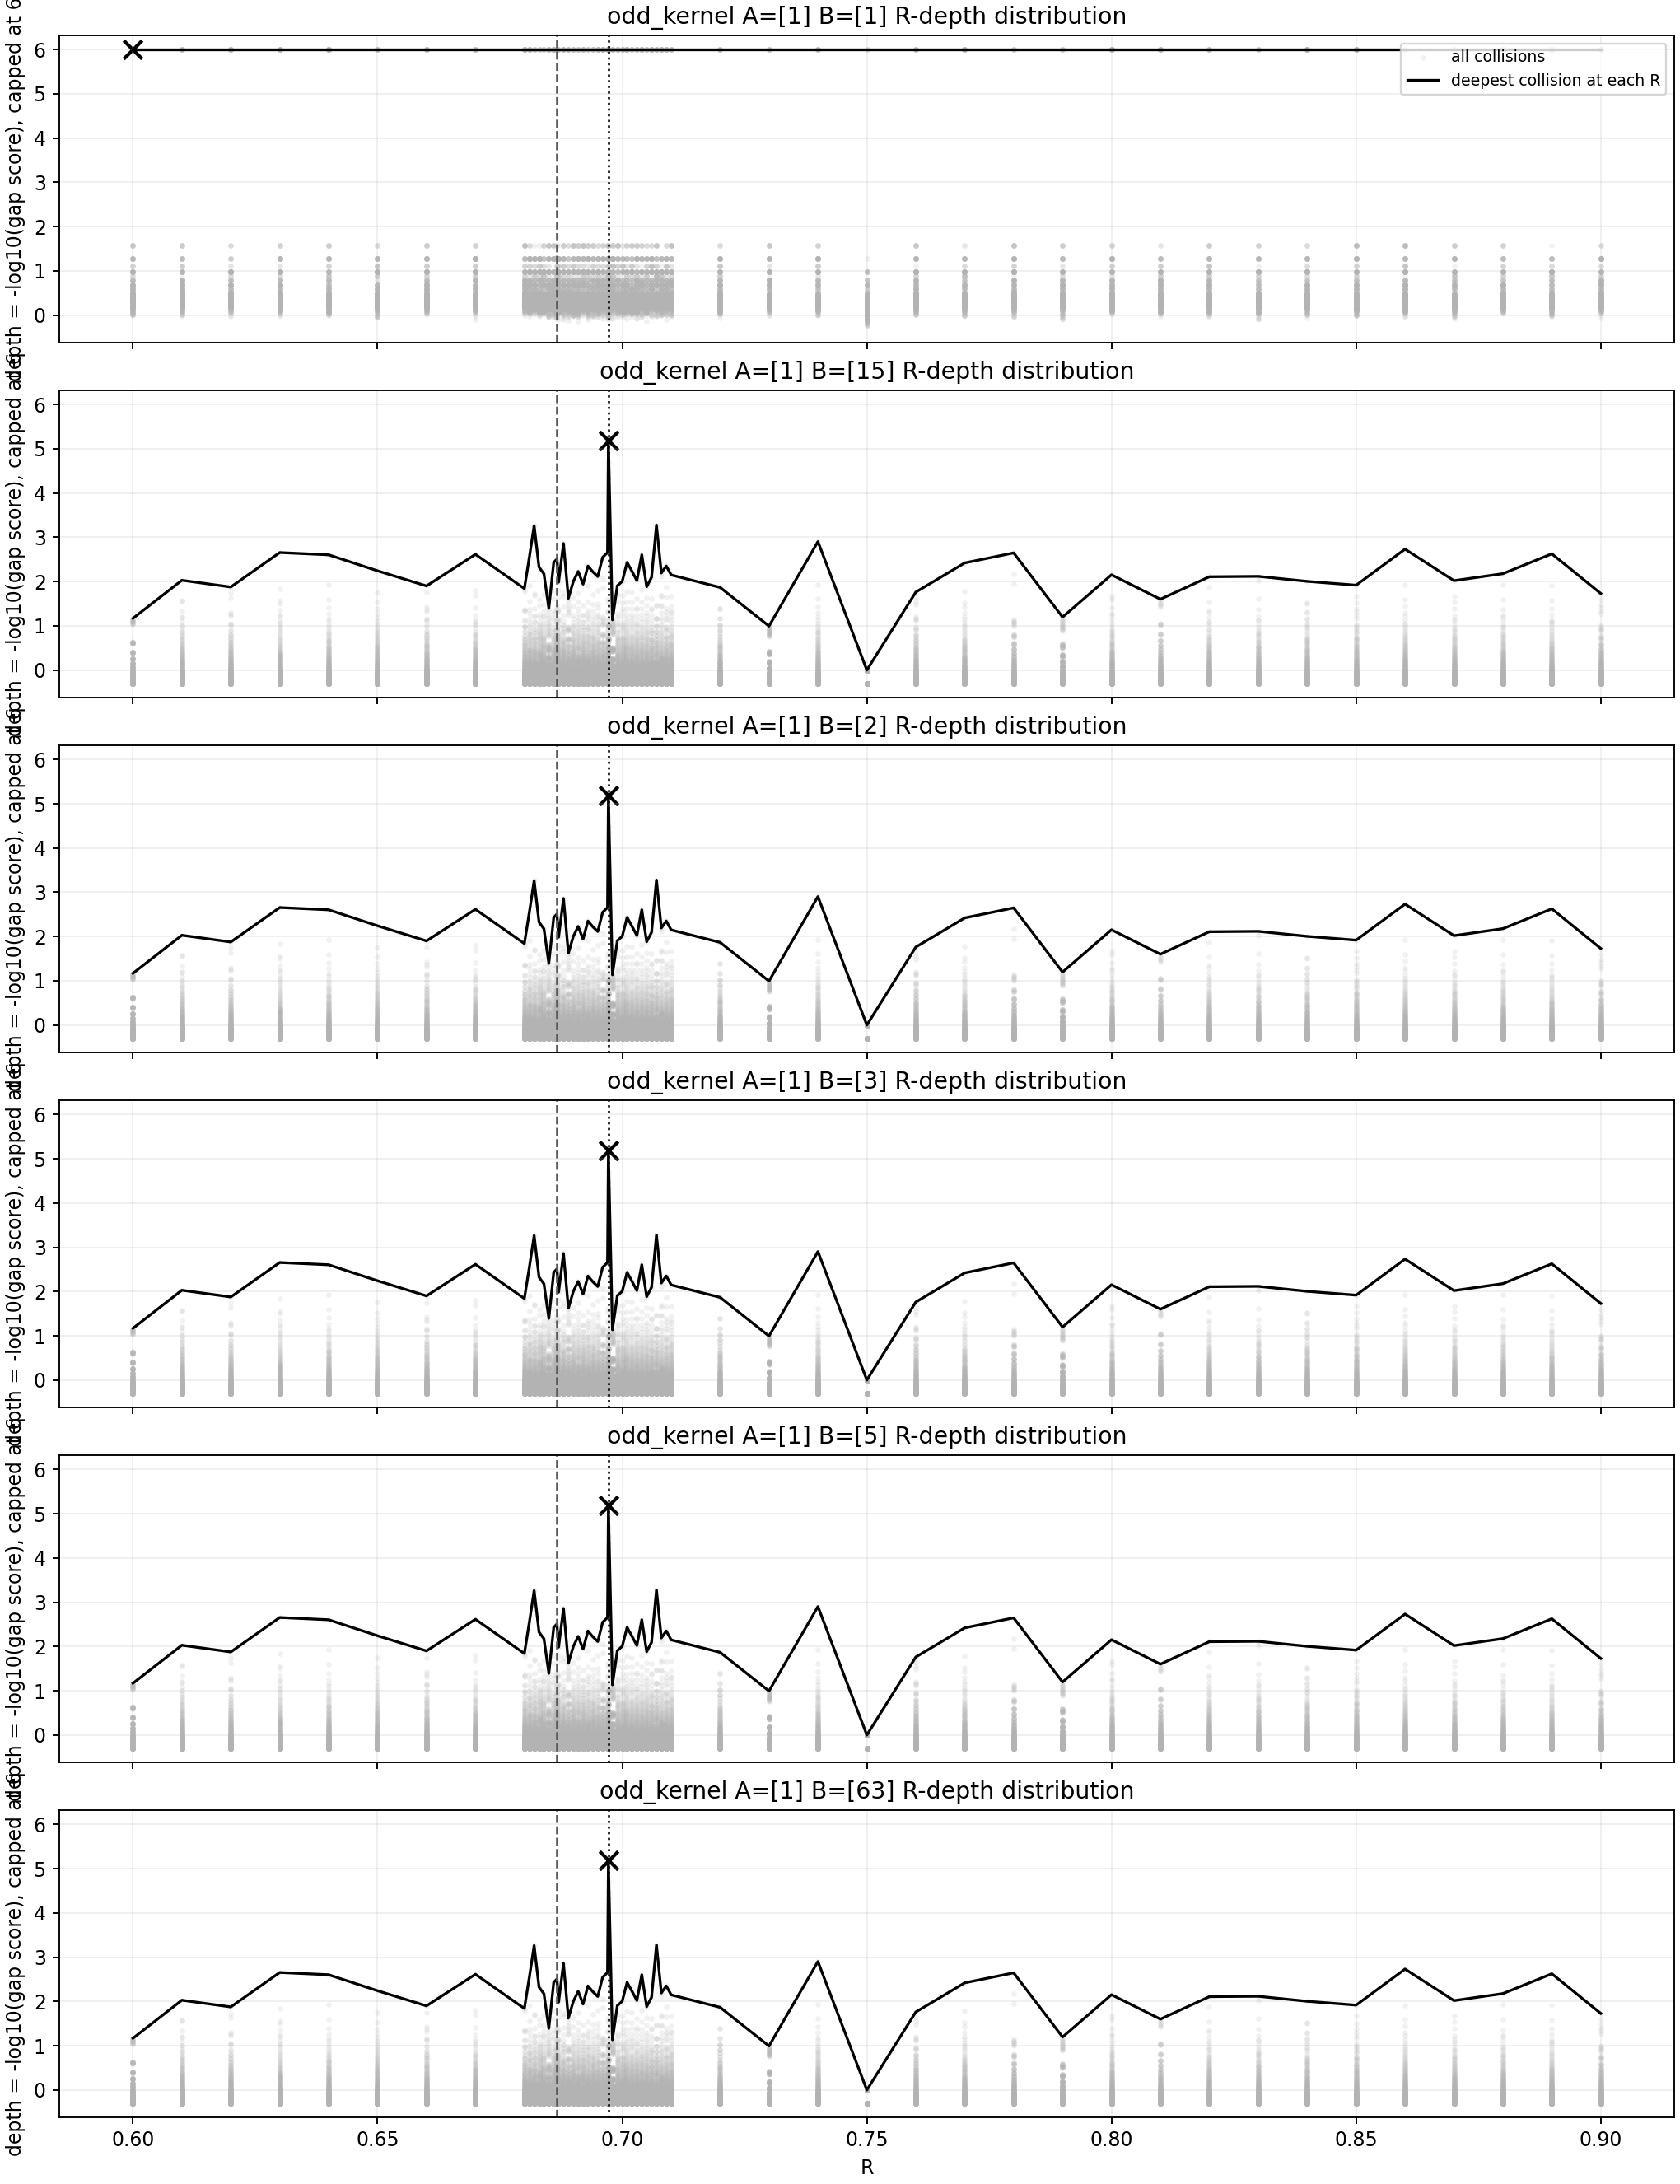
\includegraphics[keepaspectratio,alt={Exchange-weight landscape of the System A N-series}]{system_A_localization_exchange_R_sweep_result_v1/odd_kernel_N_1_2_3_5_15_63_gap_depth_distribution_overview_v1.png}}
\caption{Exchange-weight landscape of the System A N-series}
\end{figure}

\textbf{Figure 1.} System A N-series. In the single-base-harmonic
control, the landscape along the \texttt{R} axis is broad. When an
additional harmonic is placed on one side, the evaluation points
concentrate near \texttt{R\_137}, or \texttt{G\_R≈sqrt(4πalpha(0))}.

Representative values are:

{\def\LTcaptype{none} % do not increment counter
\begin{longtable}[]{@{}
  >{\raggedright\arraybackslash}p{(\linewidth - 4\tabcolsep) * \real{0.3000}}
  >{\raggedleft\arraybackslash}p{(\linewidth - 4\tabcolsep) * \real{0.4000}}
  >{\raggedright\arraybackslash}p{(\linewidth - 4\tabcolsep) * \real{0.3000}}@{}}
\toprule\noalign{}
\begin{minipage}[b]{\linewidth}\raggedright
Condition
\end{minipage} & \begin{minipage}[b]{\linewidth}\raggedleft
\texttt{R\_star\_joint}
\end{minipage} & \begin{minipage}[b]{\linewidth}\raggedright
Reading
\end{minipage} \\
\midrule\noalign{}
\endhead
\bottomrule\noalign{}
\endlastfoot
\texttt{A={[}1{]},\ B={[}1{]}} & \texttt{0.6} & Same-order control. No
sharp exchange-weight concentration \\
\texttt{A={[}1{]},\ B={[}2{]}} & \texttt{0.697177879128} & Additional
harmonic present \\
\texttt{A={[}1{]},\ B={[}3{]}} & \texttt{0.697177879128} & Additional
harmonic present \\
\texttt{A={[}1{]},\ B={[}5{]}} & \texttt{0.697177879128} & Additional
harmonic present \\
\texttt{A={[}1{]},\ B={[}15{]}} & \texttt{0.697177879128} & Additional
harmonic present \\
\texttt{A={[}1{]},\ B={[}63{]}} & \texttt{0.697177879128} & Additional
harmonic present \\
\end{longtable}
}

The result indicates that the key condition is not odd harmonics
themselves, but the existence of at least one additional harmonic degree
of freedom.

\subsubsection{3.2 Odd, Even, and Mixed Harmonic
Packets}\label{odd-even-and-mixed-harmonic-packets}

Next, the B-side harmonic packet was varied.

\begin{Shaded}
\begin{Highlighting}[]
\NormalTok{even packet:}
\NormalTok{  B=[1,2,4,6]}

\NormalTok{alternating packet 1:}
\NormalTok{  B=[1,2,3,4,5]}

\NormalTok{alternating packet 2:}
\NormalTok{  B=[1,3,4,5,6]}
\end{Highlighting}
\end{Shaded}

All cases concentrated at \texttt{R\_star\_joint=0.697177879128}.

{\def\LTcaptype{none} % do not increment counter
\begin{longtable}[]{@{}lr@{}}
\toprule\noalign{}
Condition & \texttt{R\_star\_joint} \\
\midrule\noalign{}
\endhead
\bottomrule\noalign{}
\endlastfoot
even packet \texttt{B={[}1,2,4,6{]}} & \texttt{0.697177879128} \\
mixed packet \texttt{B={[}1,2,3,4,5{]}} & \texttt{0.697177879128} \\
mixed packet \texttt{B={[}1,3,4,5,6{]}} & \texttt{0.697177879128} \\
\end{longtable}
}

Thus, this exchange-weight concentration is not a special property of
odd harmonics.

\subsubsection{3.3 Insensitivity to Amplitude, Phase, and
Wavelength}\label{insensitivity-to-amplitude-phase-and-wavelength}

The amplitude, phase, and wavelength of the additional B-side harmonic
were then varied.

For the amplitude test, \texttt{R\_star\_joint} was maintained even when
the additional harmonic weight was strongly reduced.

{\def\LTcaptype{none} % do not increment counter
\begin{longtable}[]{@{}
  >{\raggedleft\arraybackslash}p{(\linewidth - 4\tabcolsep) * \real{0.3636}}
  >{\raggedleft\arraybackslash}p{(\linewidth - 4\tabcolsep) * \real{0.3636}}
  >{\raggedright\arraybackslash}p{(\linewidth - 4\tabcolsep) * \real{0.2727}}@{}}
\toprule\noalign{}
\begin{minipage}[b]{\linewidth}\raggedleft
additional harmonic weight
\end{minipage} & \begin{minipage}[b]{\linewidth}\raggedleft
\texttt{R\_star\_joint}
\end{minipage} & \begin{minipage}[b]{\linewidth}\raggedright
Reading
\end{minipage} \\
\midrule\noalign{}
\endhead
\bottomrule\noalign{}
\endlastfoot
\texttt{0.5} & \texttt{0.697177879128} & maintained \\
\texttt{0.1} & \texttt{0.697177879128} & maintained \\
\texttt{0.001} & \texttt{0.697177879128} & maintained \\
\texttt{0.0001} & \texttt{0.697177879128} & maintained \\
\texttt{0.000001} & \texttt{0.697177879128} & some indicators fluctuate,
but joint value maintained \\
\texttt{0} & \texttt{0.6} & no exchange-weight concentration \\
\end{longtable}
}

When the phase was shifted by 10\% or 30\%,
\texttt{R\_star\_joint=0.697177879128} was maintained.

When the wavelength was shifted by 3\%, 10\%, or 30\%, the same
\texttt{R\_star\_joint} was maintained.

This shows that the exchange-weight concentration is not determined only
by harmonic amplitude, phase alignment, or exact wavelength matching.

The reading adopted in this paper is:

\begin{Shaded}
\begin{Highlighting}[]
\NormalTok{The concentration of the exchange weight does not require oddness.}
\NormalTok{It does not require exact amplitude matching.}
\NormalTok{It does not require exact phase matching.}
\NormalTok{It does not require exact wavelength matching.}

\NormalTok{The presence of at least one additional harmonic degree of freedom}
\NormalTok{sets up the exchange{-}weight landscape for localization exchange.}
\end{Highlighting}
\end{Shaded}

\begin{center}\rule{0.5\linewidth}{0.5pt}\end{center}

\subsection{4. System B {[}5,8{]}: Exchange-Weight Landscape of the Gray
Metastable
Interface}\label{system-b-58-exchange-weight-landscape-of-the-gray-metastable-interface}

System B uses the white-cat, black-cat, and gray-cat metastable
interface of self-reference {[}5{]} as its base, and sweeps \texttt{R}
according to the specification in self-reference {[}8{]}.

The state is classified by

\begin{Shaded}
\begin{Highlighting}[]
\NormalTok{S = p\_A {-} p\_B.}
\end{Highlighting}
\end{Shaded}

The quality of the gray metastable phase is evaluated by

\begin{Shaded}
\begin{Highlighting}[]
\NormalTok{gray\_error = |S\_mean| + |S\_amp {-} S\_amp\_target| + S\_drift + phase\_penalty}
\NormalTok{gray\_depth = {-}log10(gray\_error)}
\end{Highlighting}
\end{Shaded}

where

\begin{Shaded}
\begin{Highlighting}[]
\NormalTok{S\_amp\_target = 0.02.}
\end{Highlighting}
\end{Shaded}

In the initial broad and local sweeps, several candidate points such as
\texttt{R=0.683}, \texttt{R=0.700}, and \texttt{R=0.697177879128}
appeared. This indicates that the gray metastable interface has a
multi-peak exchange-weight landscape along the \texttt{R} axis rather
than a single peak.

\begin{figure}
\centering
\pandocbounded{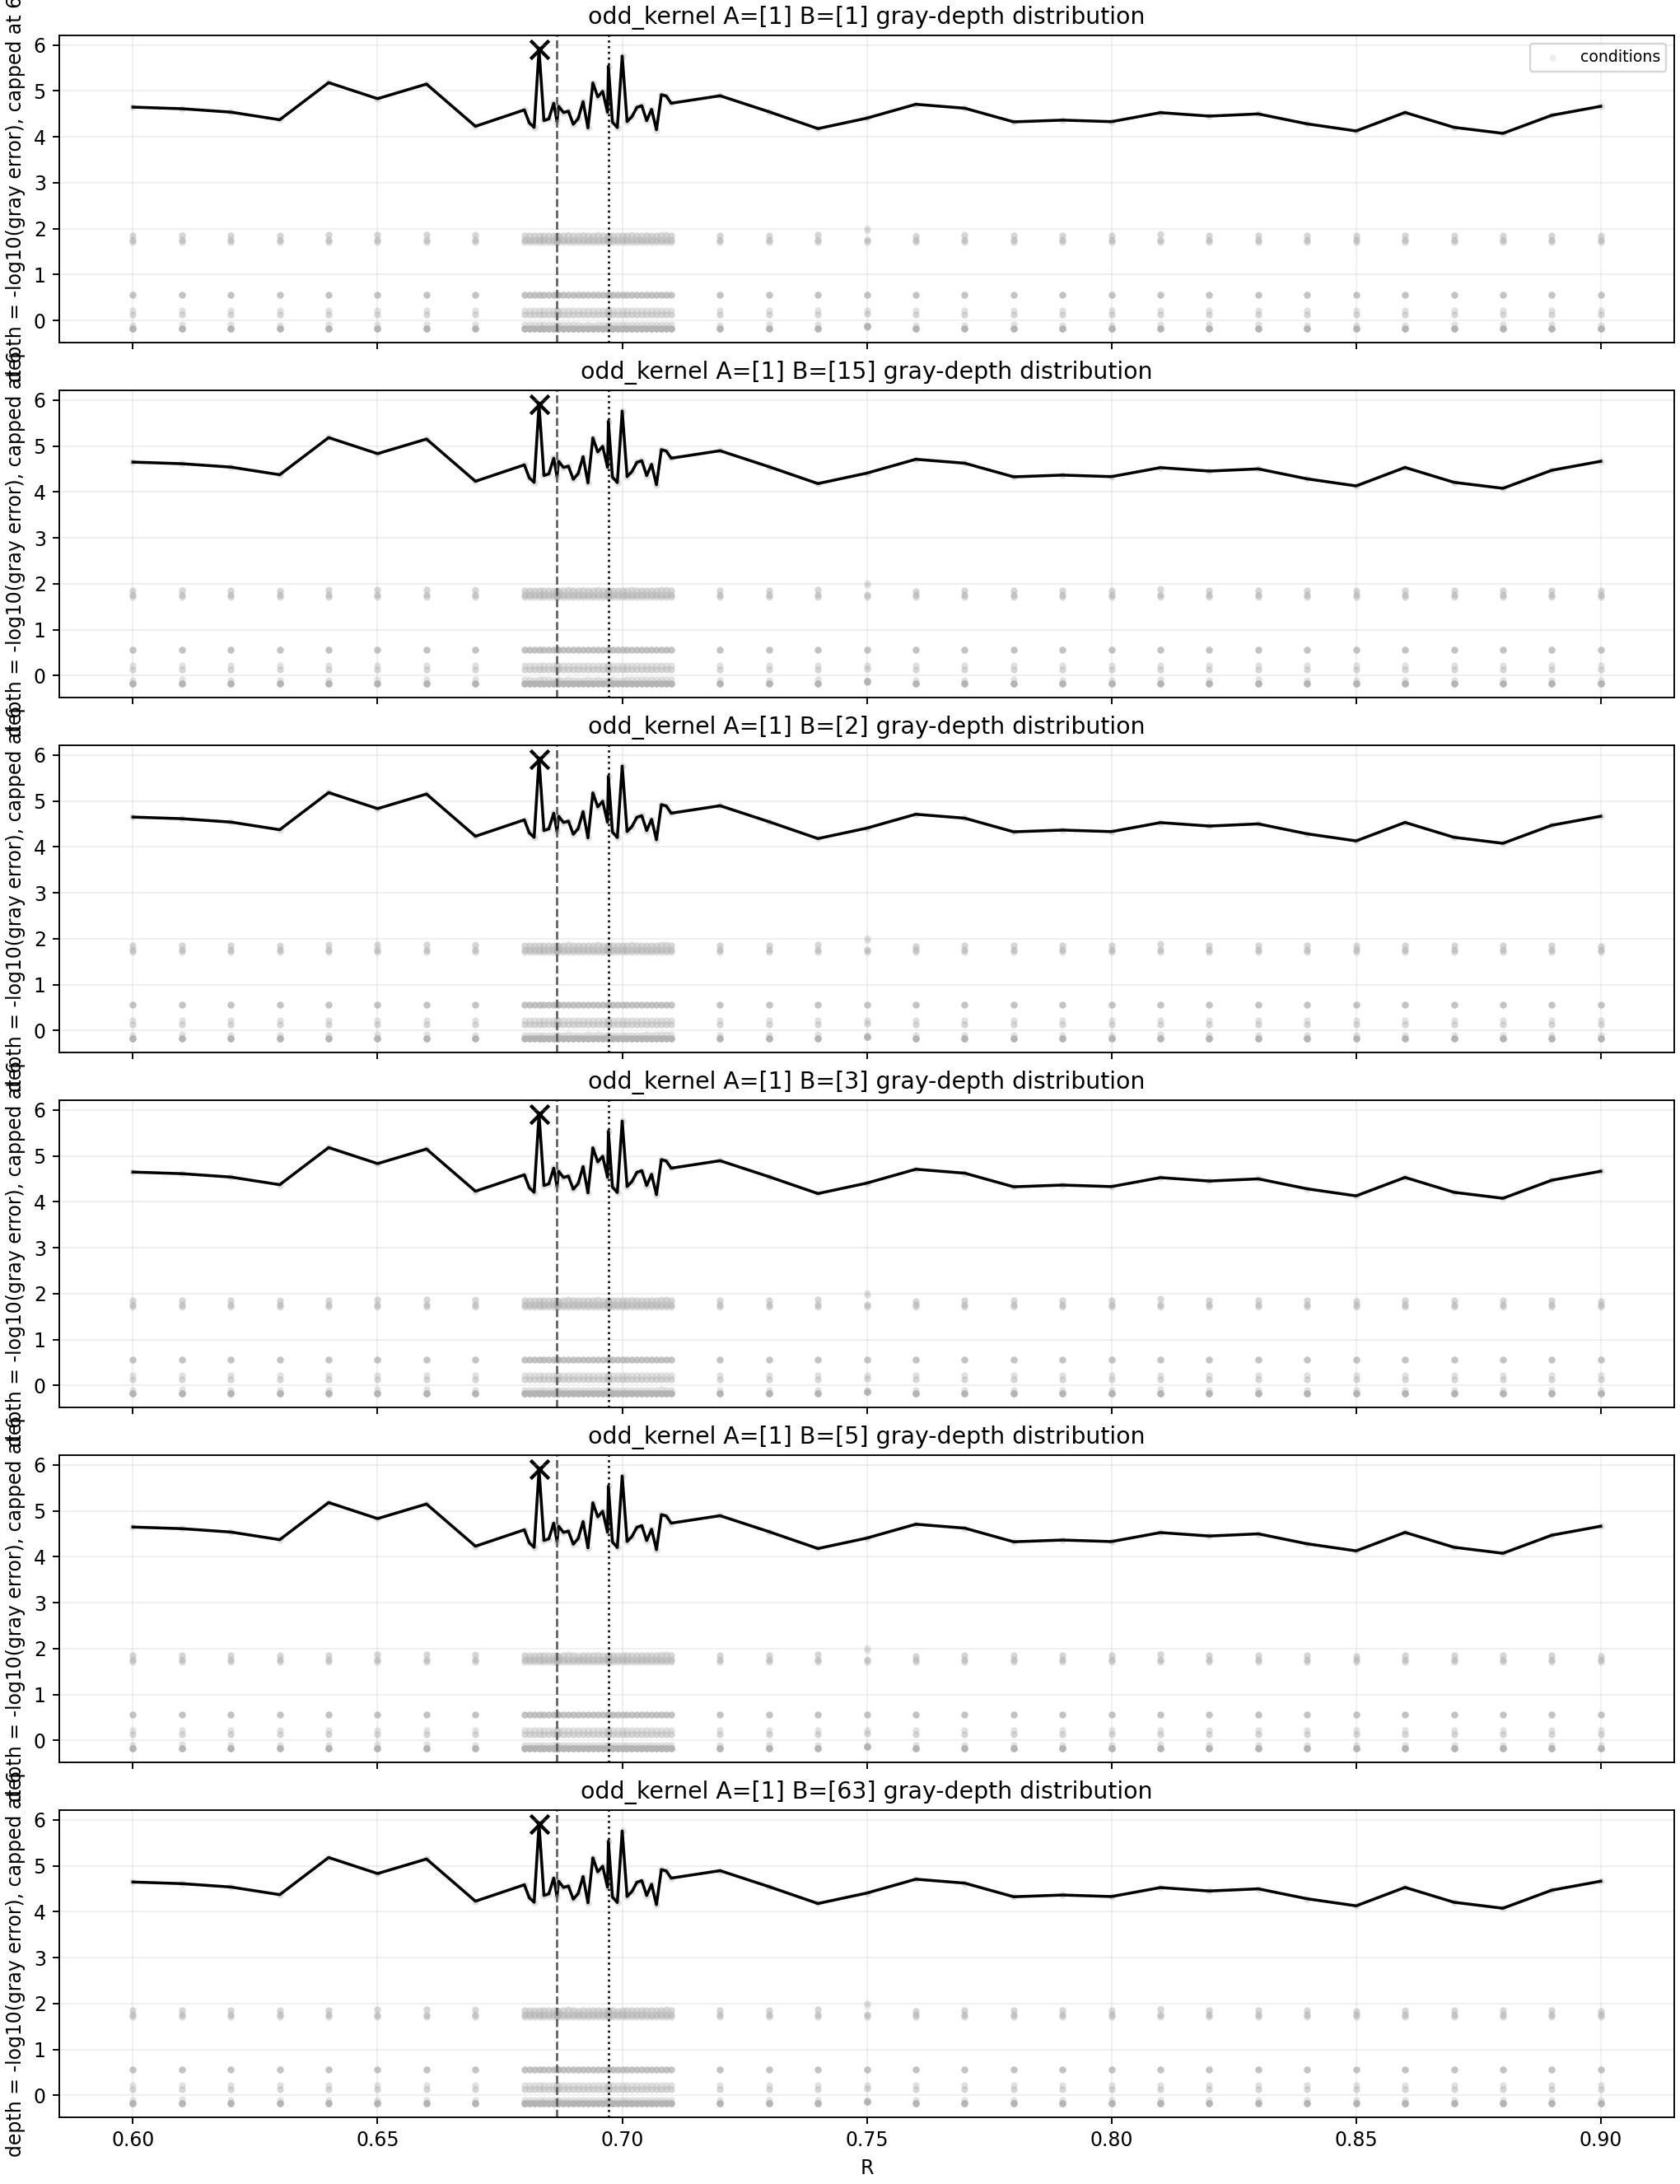
\includegraphics[keepaspectratio,alt={Initial exchange-weight landscape of System B}]{system_B_gray_cat_metastable_R_sweep_result_v1/system_B_odd_kernel_N_1_2_3_5_15_63_gray_depth_distribution_overview_v1.png}}
\caption{Initial exchange-weight landscape of System B}
\end{figure}

\textbf{Figure 2.} Initial exchange-weight landscape of System B. The
gray metastable interface has several local peaks rather than a single
value of \texttt{R}.

However, the initial experiment used a coarse \texttt{R} range and might
over-detect candidate points. Therefore, a minimized v5 implementation
was used to scan a broad range with a uniform step.

\begin{center}\rule{0.5\linewidth}{0.5pt}\end{center}

\subsection{5. Full-Range R Sweep with the Minimal v5
Implementation}\label{full-range-r-sweep-with-the-minimal-v5-implementation}

\subsubsection{5.1 Experimental
Conditions}\label{experimental-conditions}

The v5 implementation removes unnecessary outputs for the investigation
and reads only the gray-metastable depth for a specified \texttt{R}.

The full-range sweep conditions were:

{\def\LTcaptype{none} % do not increment counter
\begin{longtable}[]{@{}lr@{}}
\toprule\noalign{}
Item & Value \\
\midrule\noalign{}
\endhead
\bottomrule\noalign{}
\endlastfoot
\texttt{min\_R} & \texttt{0.68660290255614798} \\
\texttt{max\_R} & \texttt{0.70246536756843059} \\
\texttt{delta\_R} & \texttt{0.0000001} \\
\texttt{n\_R} & \texttt{158625} \\
\texttt{steps} & \texttt{1024} \\
\texttt{min\_steps} & \texttt{256} \\
\texttt{early\_stop\_patience} & \texttt{20} \\
\texttt{phi\_mode} & \texttt{zero} \\
\end{longtable}
}

This range includes the neighborhood of \texttt{R\_MZ} on the
high-energy side and sufficiently covers \texttt{R\_low} on the
low-energy side.

\subsubsection{5.2 Candidate Bands}\label{candidate-bands}

In the full-range sweep, candidate points were grouped into continuous
bands. Seven candidate bands were obtained.

{\def\LTcaptype{none} % do not increment counter
\begin{longtable}[]{@{}
  >{\raggedleft\arraybackslash}p{(\linewidth - 12\tabcolsep) * \real{0.1429}}
  >{\raggedleft\arraybackslash}p{(\linewidth - 12\tabcolsep) * \real{0.1429}}
  >{\raggedleft\arraybackslash}p{(\linewidth - 12\tabcolsep) * \real{0.1429}}
  >{\raggedleft\arraybackslash}p{(\linewidth - 12\tabcolsep) * \real{0.1429}}
  >{\raggedleft\arraybackslash}p{(\linewidth - 12\tabcolsep) * \real{0.1429}}
  >{\raggedleft\arraybackslash}p{(\linewidth - 12\tabcolsep) * \real{0.1429}}
  >{\raggedleft\arraybackslash}p{(\linewidth - 12\tabcolsep) * \real{0.1429}}@{}}
\toprule\noalign{}
\begin{minipage}[b]{\linewidth}\raggedleft
Rank
\end{minipage} & \begin{minipage}[b]{\linewidth}\raggedleft
R\_start
\end{minipage} & \begin{minipage}[b]{\linewidth}\raggedleft
R\_end
\end{minipage} & \begin{minipage}[b]{\linewidth}\raggedleft
peak\_R
\end{minipage} & \begin{minipage}[b]{\linewidth}\raggedleft
depth
\end{minipage} & \begin{minipage}[b]{\linewidth}\raggedleft
normalized depth
\end{minipage} & \begin{minipage}[b]{\linewidth}\raggedleft
converted \texttt{1/alpha}
\end{minipage} \\
\midrule\noalign{}
\endhead
\bottomrule\noalign{}
\endlastfoot
1 & \texttt{0.697060302556148} & \texttt{0.697625902556148} &
\texttt{0.697177902556148} & \texttt{9.08320492077} & \texttt{1.000000}
& \texttt{137.036020287643} \\
2 & \texttt{0.688146602556148} & \texttt{0.688539502556148} &
\texttt{0.688363902556148} & \texttt{8.84756342227} & \texttt{0.974057}
& \texttt{129.394062925467} \\
3 & \texttt{0.692118902556148} & \texttt{0.692927402556148} &
\texttt{0.692852802556148} & \texttt{5.84993869466} & \texttt{0.644039}
& \texttt{133.203841605880} \\
4 & \texttt{0.701163902556148} & \texttt{0.701587402556148} &
\texttt{0.701489902556148} & \texttt{5.83931992499} & \texttt{0.642870}
& \texttt{141.023604736761} \\
5 & \texttt{0.686752802556148} & \texttt{0.687177802556148} &
\texttt{0.687009702556148} & \texttt{5.81816843379} & \texttt{0.640541}
& \texttt{128.276799088738} \\
6 & \texttt{0.698514602556148} & \texttt{0.699071002556148} &
\texttt{0.698893702556148} & \texttt{5.74438302514} & \texttt{0.632418}
& \texttt{138.602220120334} \\
7 & \texttt{0.692068702556148} & \texttt{0.692108002556148} &
\texttt{0.692075802556148} & \texttt{4.61388675601} & \texttt{0.507958}
& \texttt{132.532450378510} \\
\end{longtable}
}

\begin{figure}
\centering
\pandocbounded{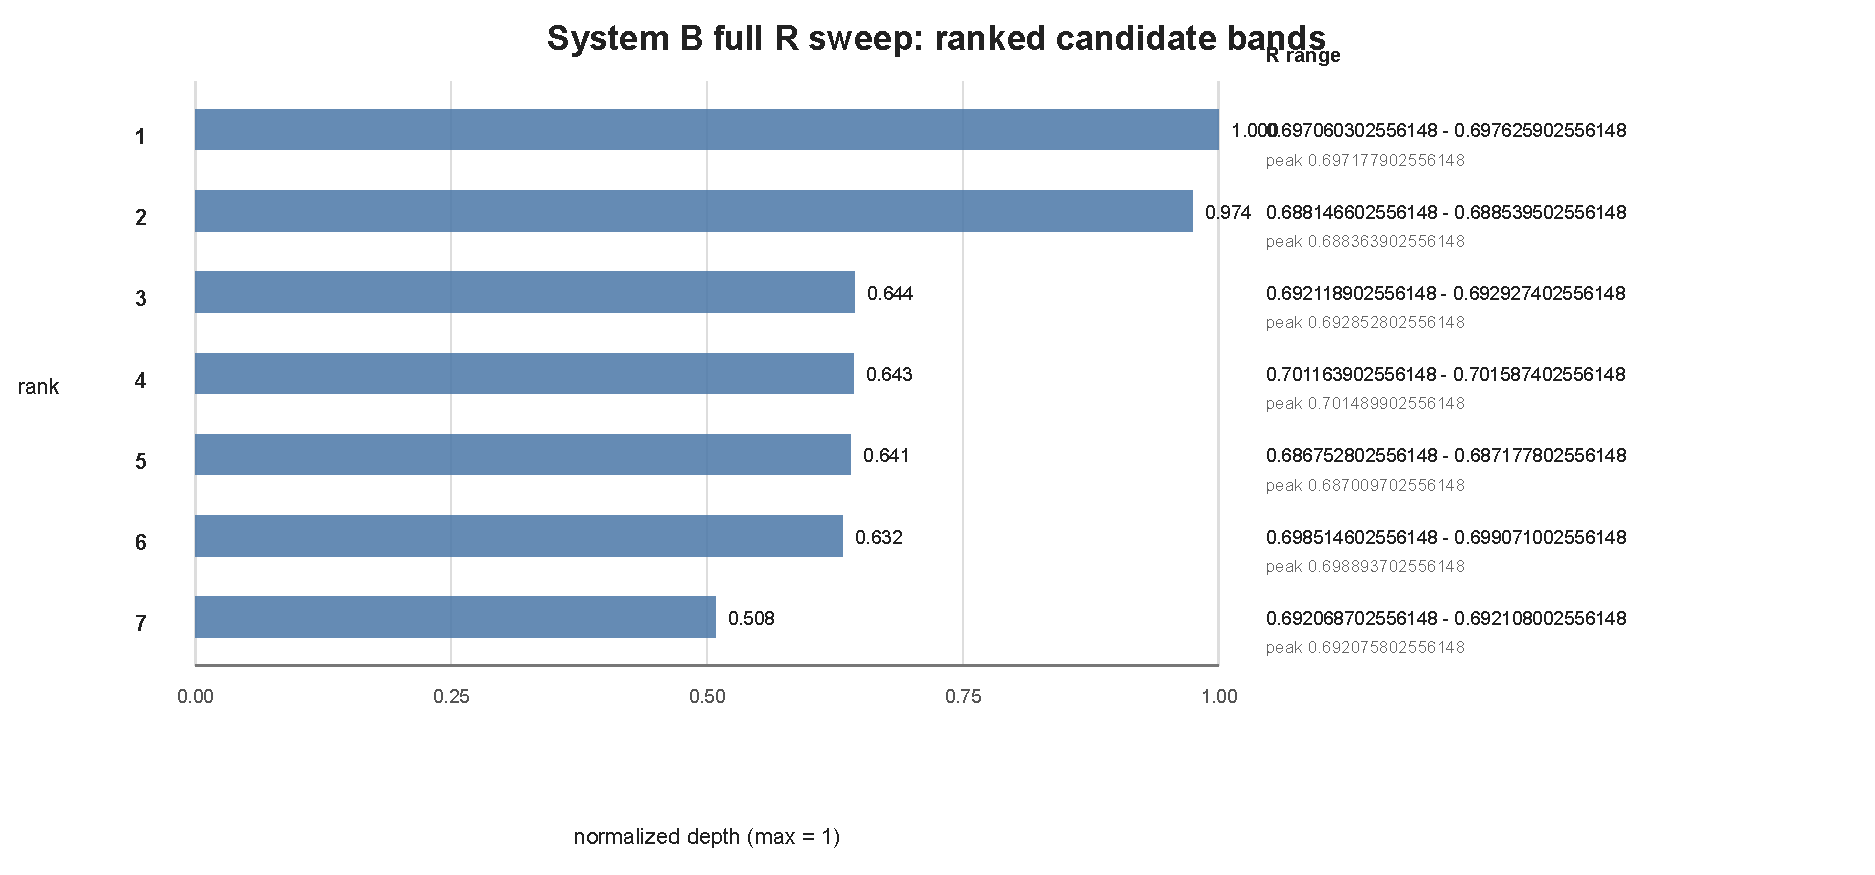
\includegraphics[keepaspectratio,alt={Candidate band ranking}]{system_B_full_R_sweep_ranked_depth_bar_v1.pdf}}
\caption{Candidate band ranking}
\end{figure}

\textbf{Figure 3.} Candidate bands detected in the full-range sweep.
Candidate bands 1 and 2 are deep, while the remaining candidate bands
are clearly shallower.

\subsubsection{5.3 Full-Range Figure}\label{full-range-figure}

In the full-range figure, candidate bands 1 and 2 stand out sharply.

\begin{figure}
\centering
\pandocbounded{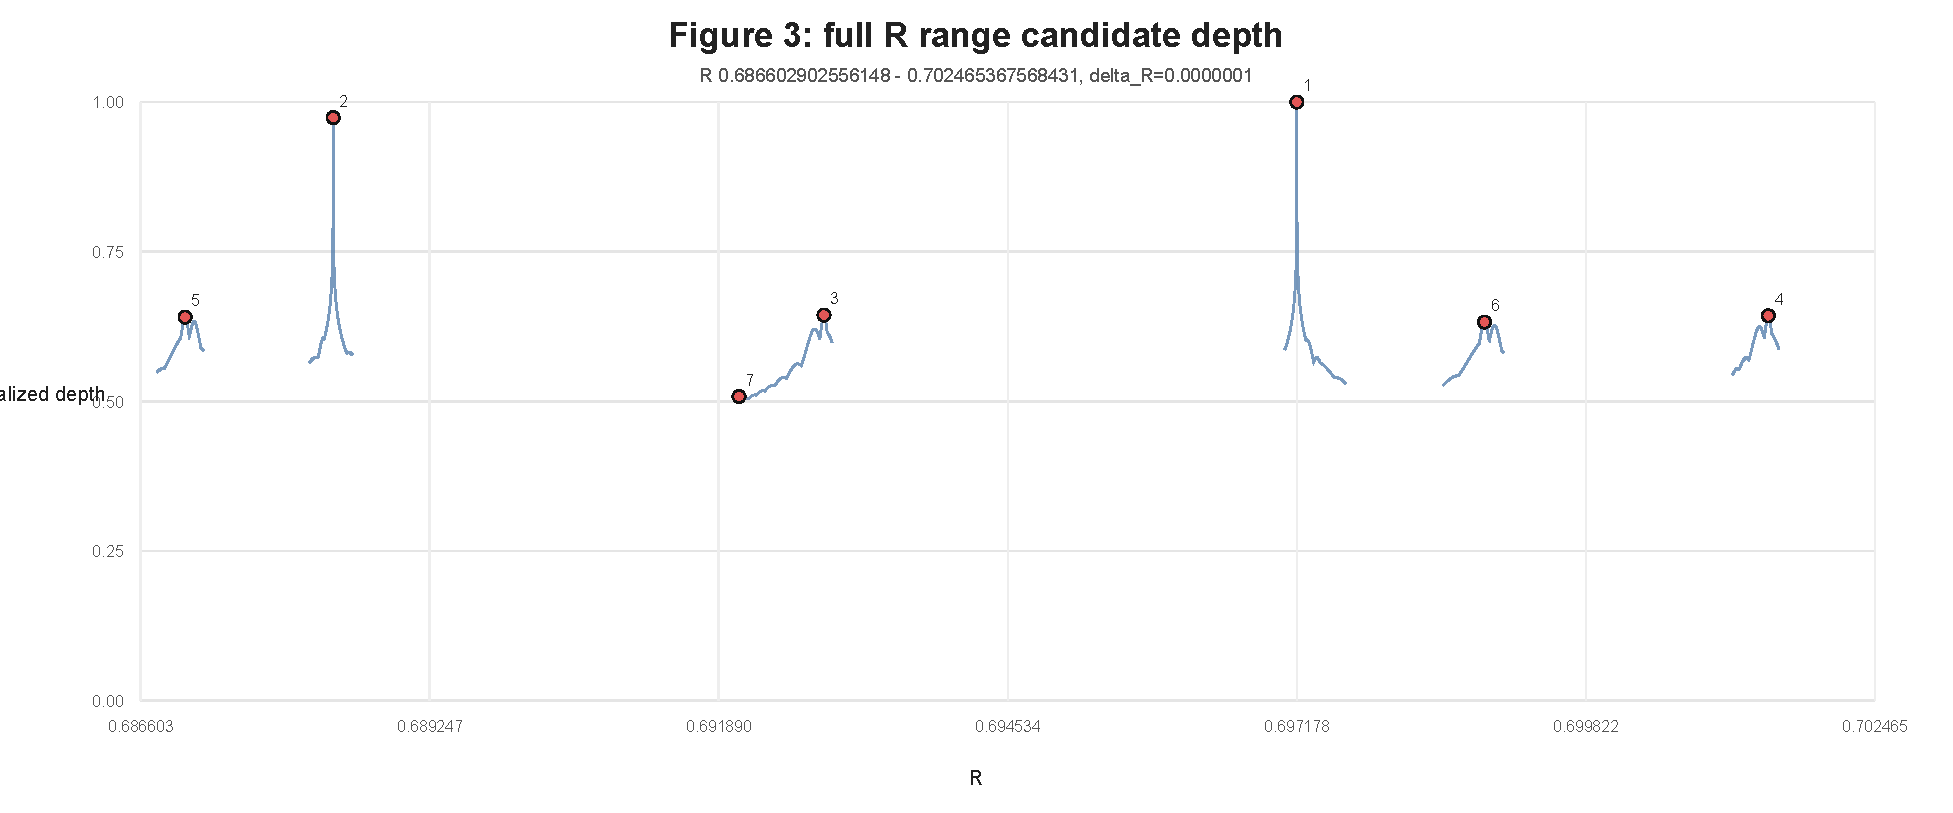
\includegraphics[keepaspectratio,alt={Full-range R sweep}]{system_B_full_R_sweep_full_range_depth_v1.pdf}}
\caption{Full-range R sweep}
\end{figure}

\textbf{Figure 4.} Full-range R sweep. Candidate band 1 is near the
point corresponding to low-energy \texttt{alpha(0)}, while candidate
band 2 is near a high-energy effective-coupling region.

\subsubsection{5.4 Candidate Band 1}\label{candidate-band-1}

The representative point of candidate band 1 is

\begin{Shaded}
\begin{Highlighting}[]
\NormalTok{R\_peak = 0.697177902556148.}
\end{Highlighting}
\end{Shaded}

The converted value from the standard-theory low-energy constant is

\begin{Shaded}
\begin{Highlighting}[]
\NormalTok{R\_low = 0.697177879231003.}
\end{Highlighting}
\end{Shaded}

The difference is

\begin{Shaded}
\begin{Highlighting}[]
\NormalTok{Delta R ≈ 2.33e{-}8,}
\end{Highlighting}
\end{Shaded}

which is within the seven-digit effective precision of the v5
experiment.

\begin{figure}
\centering
\pandocbounded{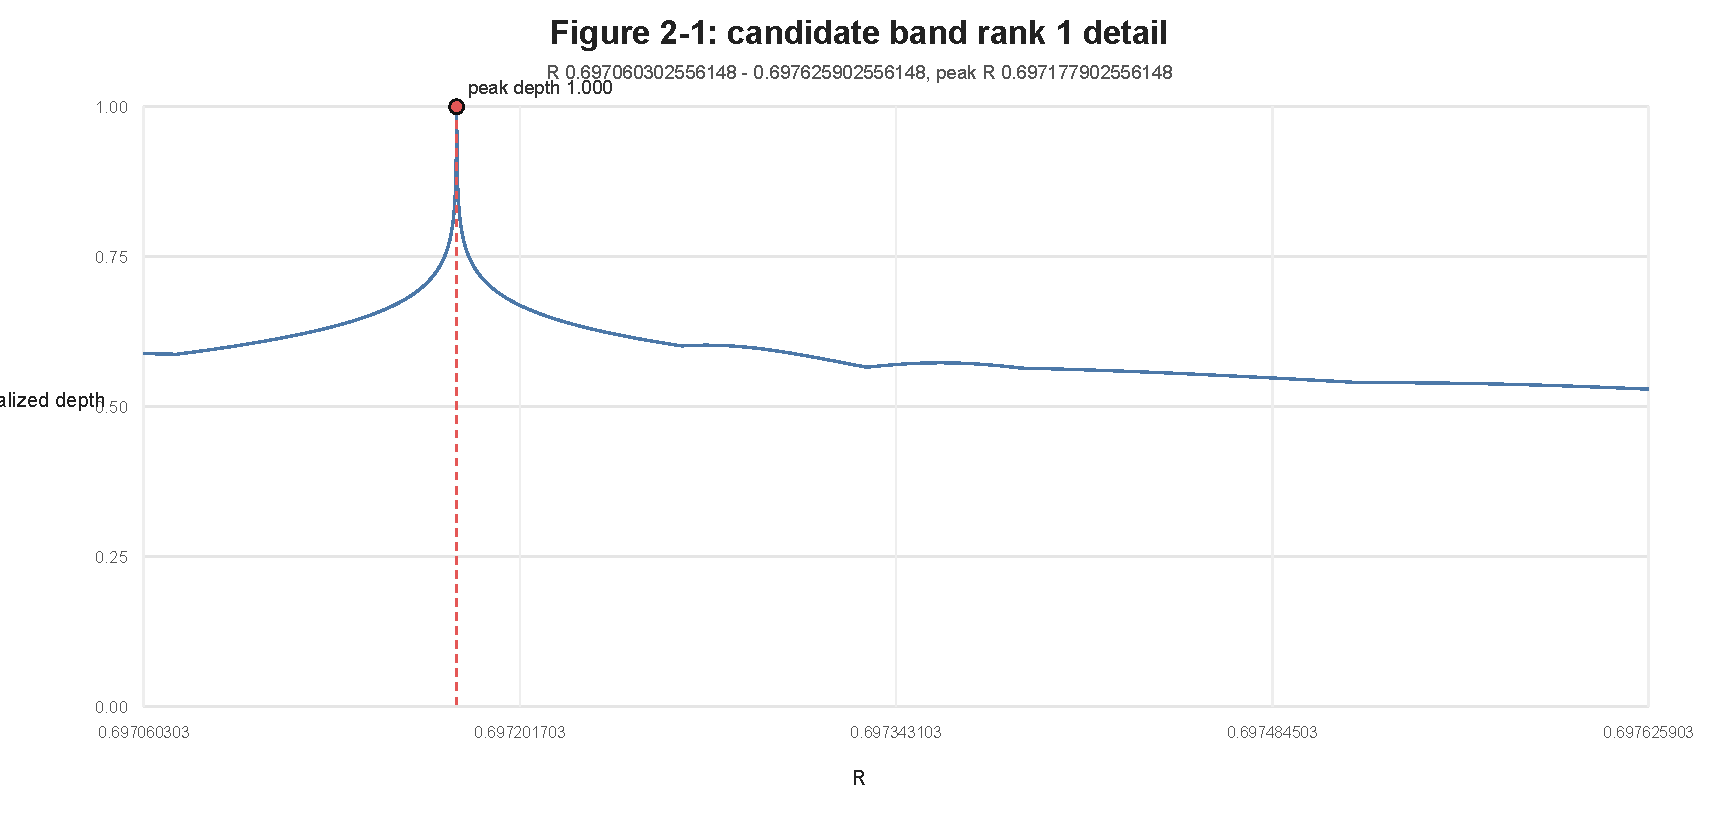
\includegraphics[keepaspectratio,alt={Candidate band 1 detail}]{system_B_full_R_sweep_band_detail_rank_01_v1.pdf}}
\caption{Candidate band 1 detail}
\end{figure}

\textbf{Figure 5.} Detail of candidate band 1. A sharp depth appears
near \texttt{R\_low}.

\subsubsection{5.5 Candidate Band 2}\label{candidate-band-2}

The representative point of candidate band 2 is

\begin{Shaded}
\begin{Highlighting}[]
\NormalTok{R\_peak = 0.688363902556148.}
\end{Highlighting}
\end{Shaded}

Converting this to \texttt{1/alpha} gives

\begin{Shaded}
\begin{Highlighting}[]
\NormalTok{1/alpha = 129.394062925467.}
\end{Highlighting}
\end{Shaded}

The standard-theory reference value at the Z-boson mass scale is

\begin{Shaded}
\begin{Highlighting}[]
\NormalTok{1/alpha(M\_Z\^{}2) = 128.946 ± 0.015}
\NormalTok{R\_MZ = 0.687822933884774.}
\end{Highlighting}
\end{Shaded}

Candidate band 2 does not coincide with the standard value within the
seven-digit precision of the v5 experiment. However, considering that
the effective precision of the high-energy standard-theory coupling is
roughly four to five digits, it has the following proximity:

\begin{Shaded}
\begin{Highlighting}[]
\NormalTok{relative difference in 1/alpha ≈ 0.35\%}
\NormalTok{relative difference in R       ≈ 0.08\%}
\end{Highlighting}
\end{Shaded}

Therefore, candidate band 2 is not treated as identical to
\texttt{alpha(M\_Z\^{}2)}, but is retained as a high-energy-side
connection candidate.

\begin{figure}
\centering
\pandocbounded{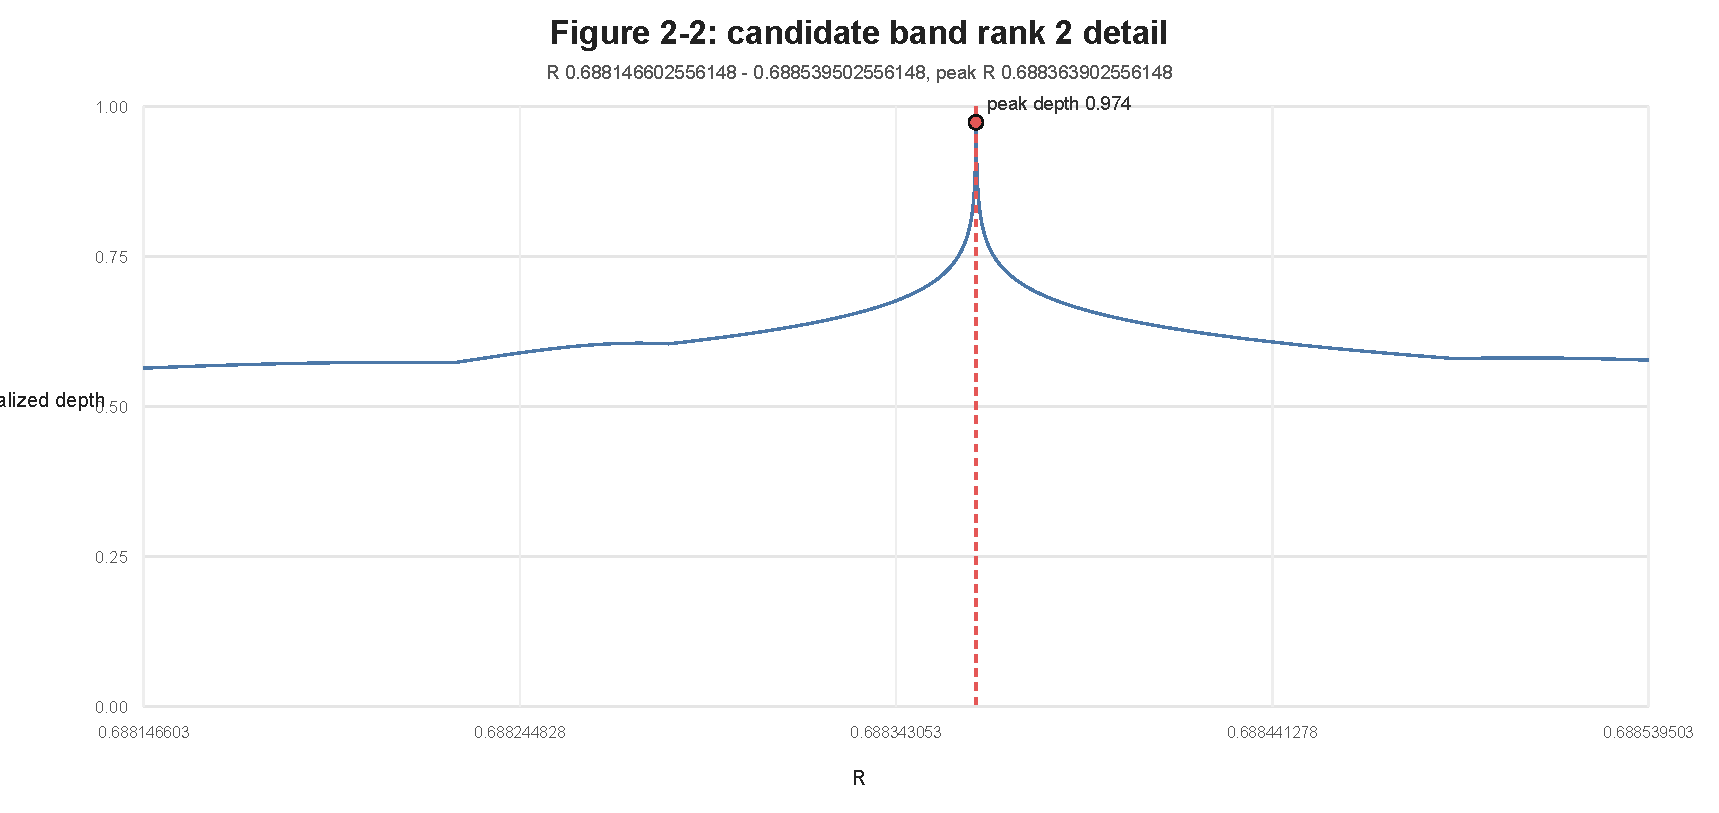
\includegraphics[keepaspectratio,alt={Candidate band 2 detail}]{system_B_full_R_sweep_band_detail_rank_02_v1.pdf}}
\caption{Candidate band 2 detail}
\end{figure}

\textbf{Figure 6.} Detail of candidate band 2. It appears as a deep
candidate band distinct from the low-energy side.

\begin{center}\rule{0.5\linewidth}{0.5pt}\end{center}

\subsection{6. Sensitivity Near the Low-Energy and High-Energy
Values}\label{sensitivity-near-the-low-energy-and-high-energy-values}

On the low-energy side, the candidate band appears stably near the
standard value.

\begin{figure}
\centering
\pandocbounded{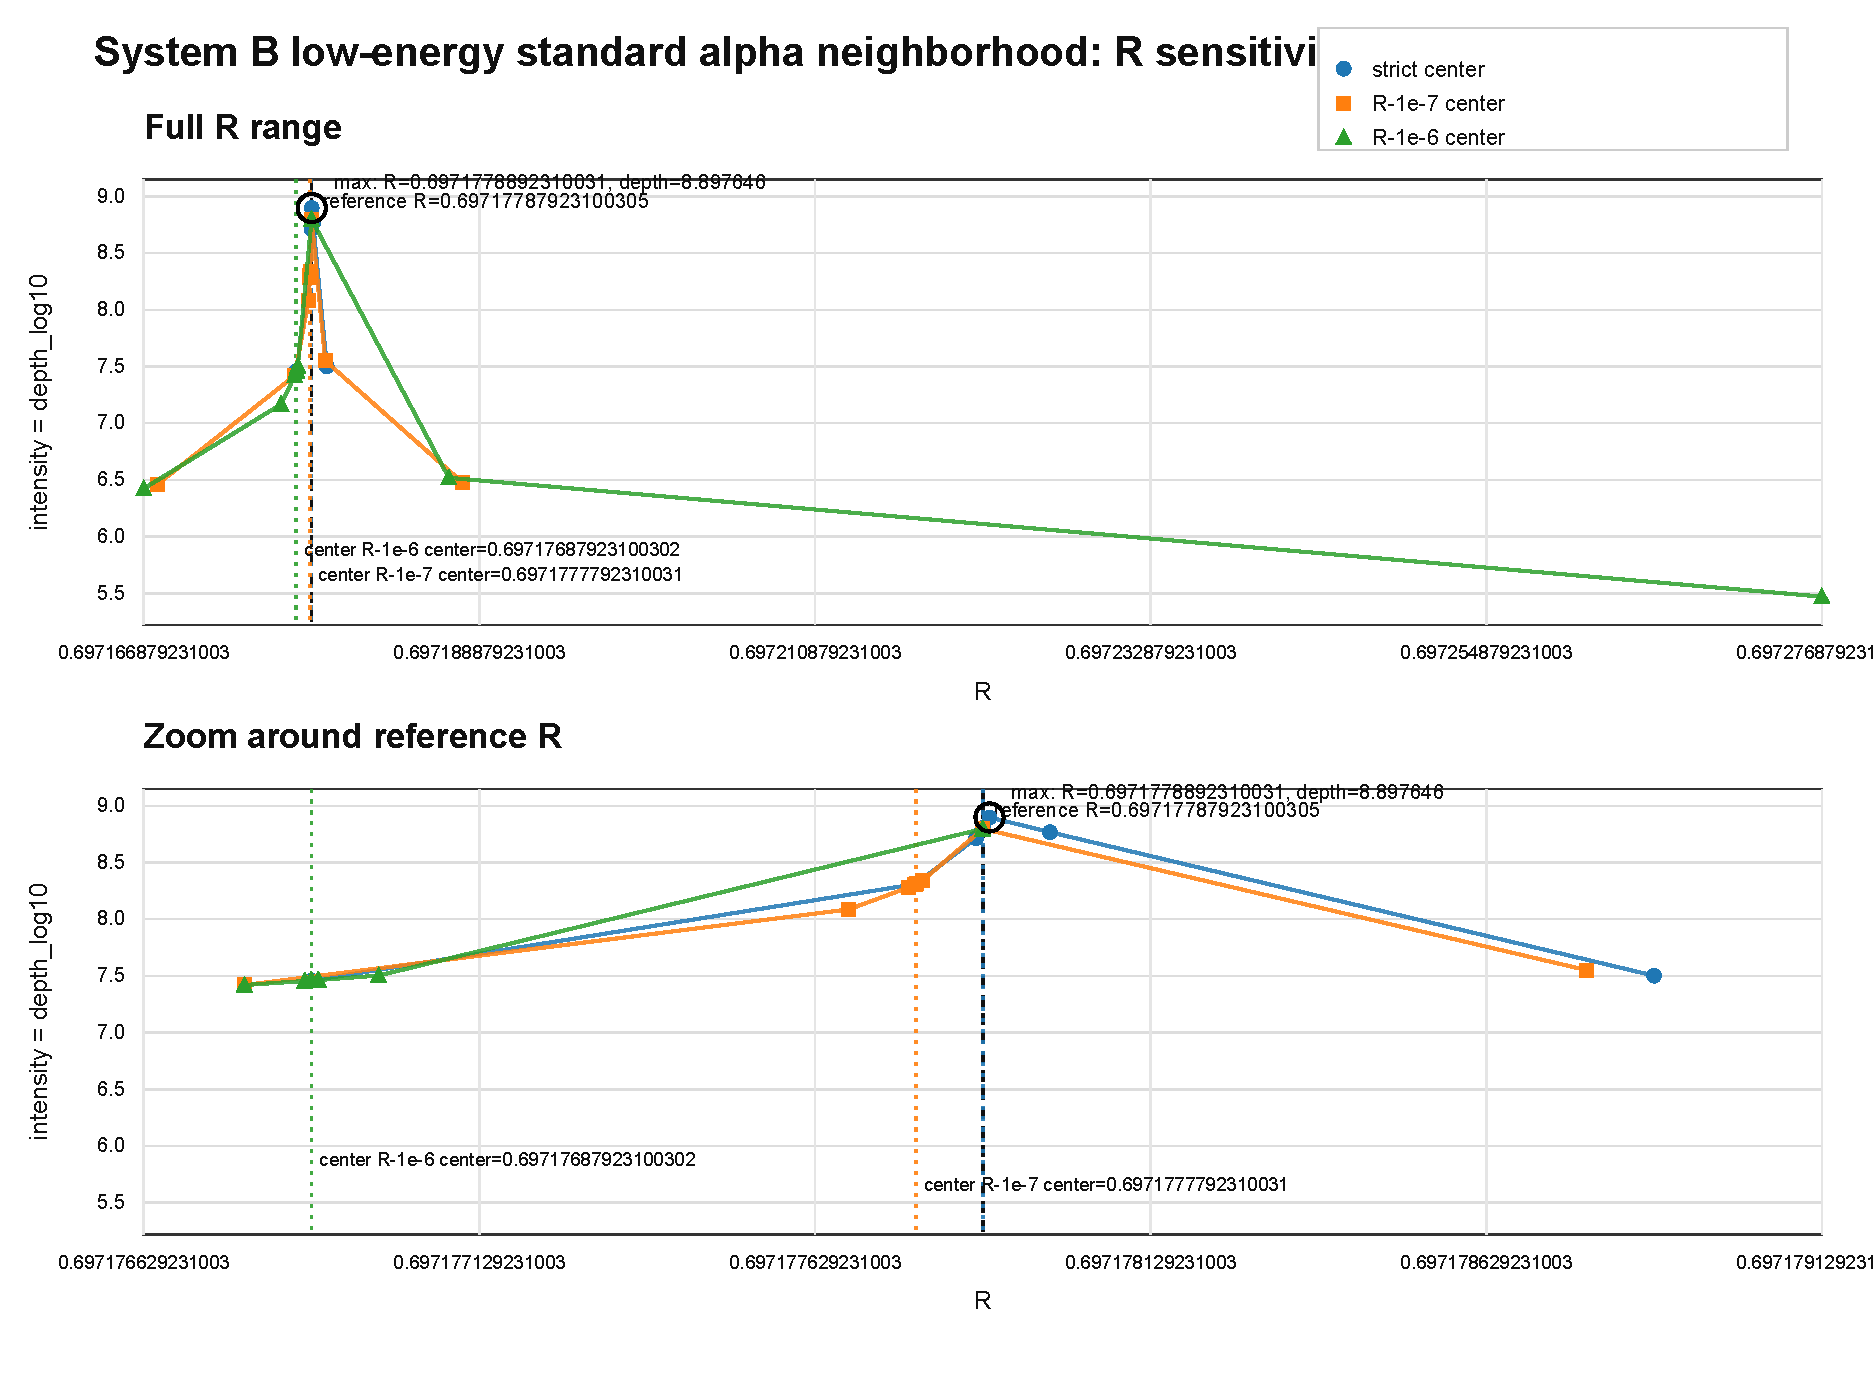
\includegraphics[keepaspectratio,alt={Low-energy alpha neighborhood}]{system_B_low_alpha_R_sensitivity_depth_v1.pdf}}
\caption{Low-energy alpha neighborhood}
\end{figure}

\textbf{Figure 7.} R sensitivity near low-energy \texttt{alpha(0)}. The
center of the candidate band remains near the standard value.

On the high-energy side, the result is better read as the appearance of
a nearby candidate band rather than as a sharply fixed point at the
standard value itself.

\begin{figure}
\centering
\pandocbounded{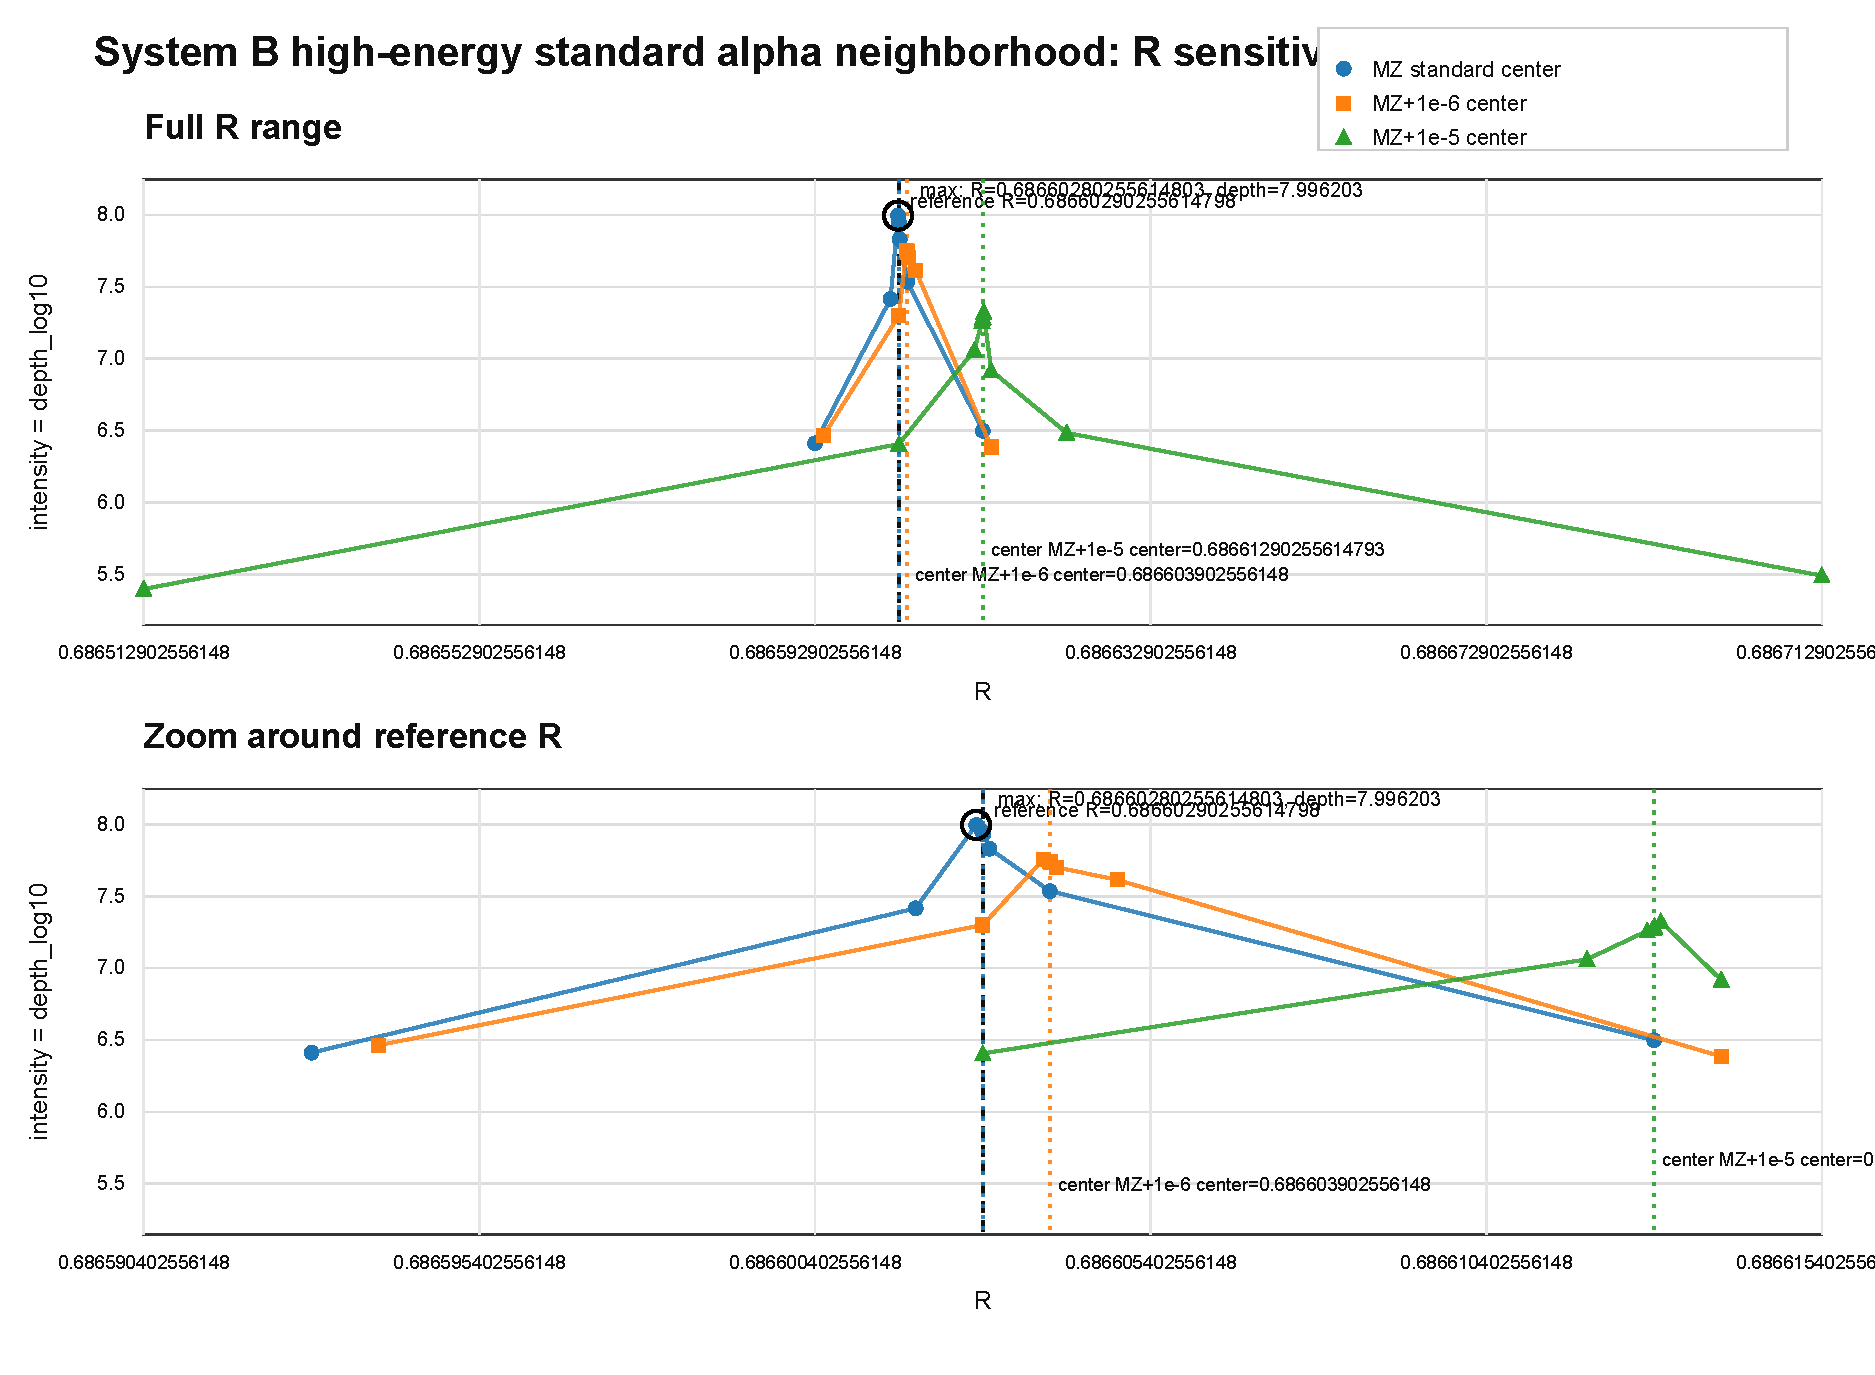
\includegraphics[keepaspectratio,alt={High-energy alpha neighborhood}]{system_B_high_alpha_R_sensitivity_depth_v1.pdf}}
\caption{High-energy alpha neighborhood}
\end{figure}

\textbf{Figure 8.} R sensitivity near high-energy
\texttt{alpha(M\_Z\^{}2)}. The point is not as sharp as the low-energy
fixed point, but a nearby candidate band appears.

In the intermediate region, no clear fixed point corresponding to a
standard value was confirmed.

\begin{figure}
\centering
\pandocbounded{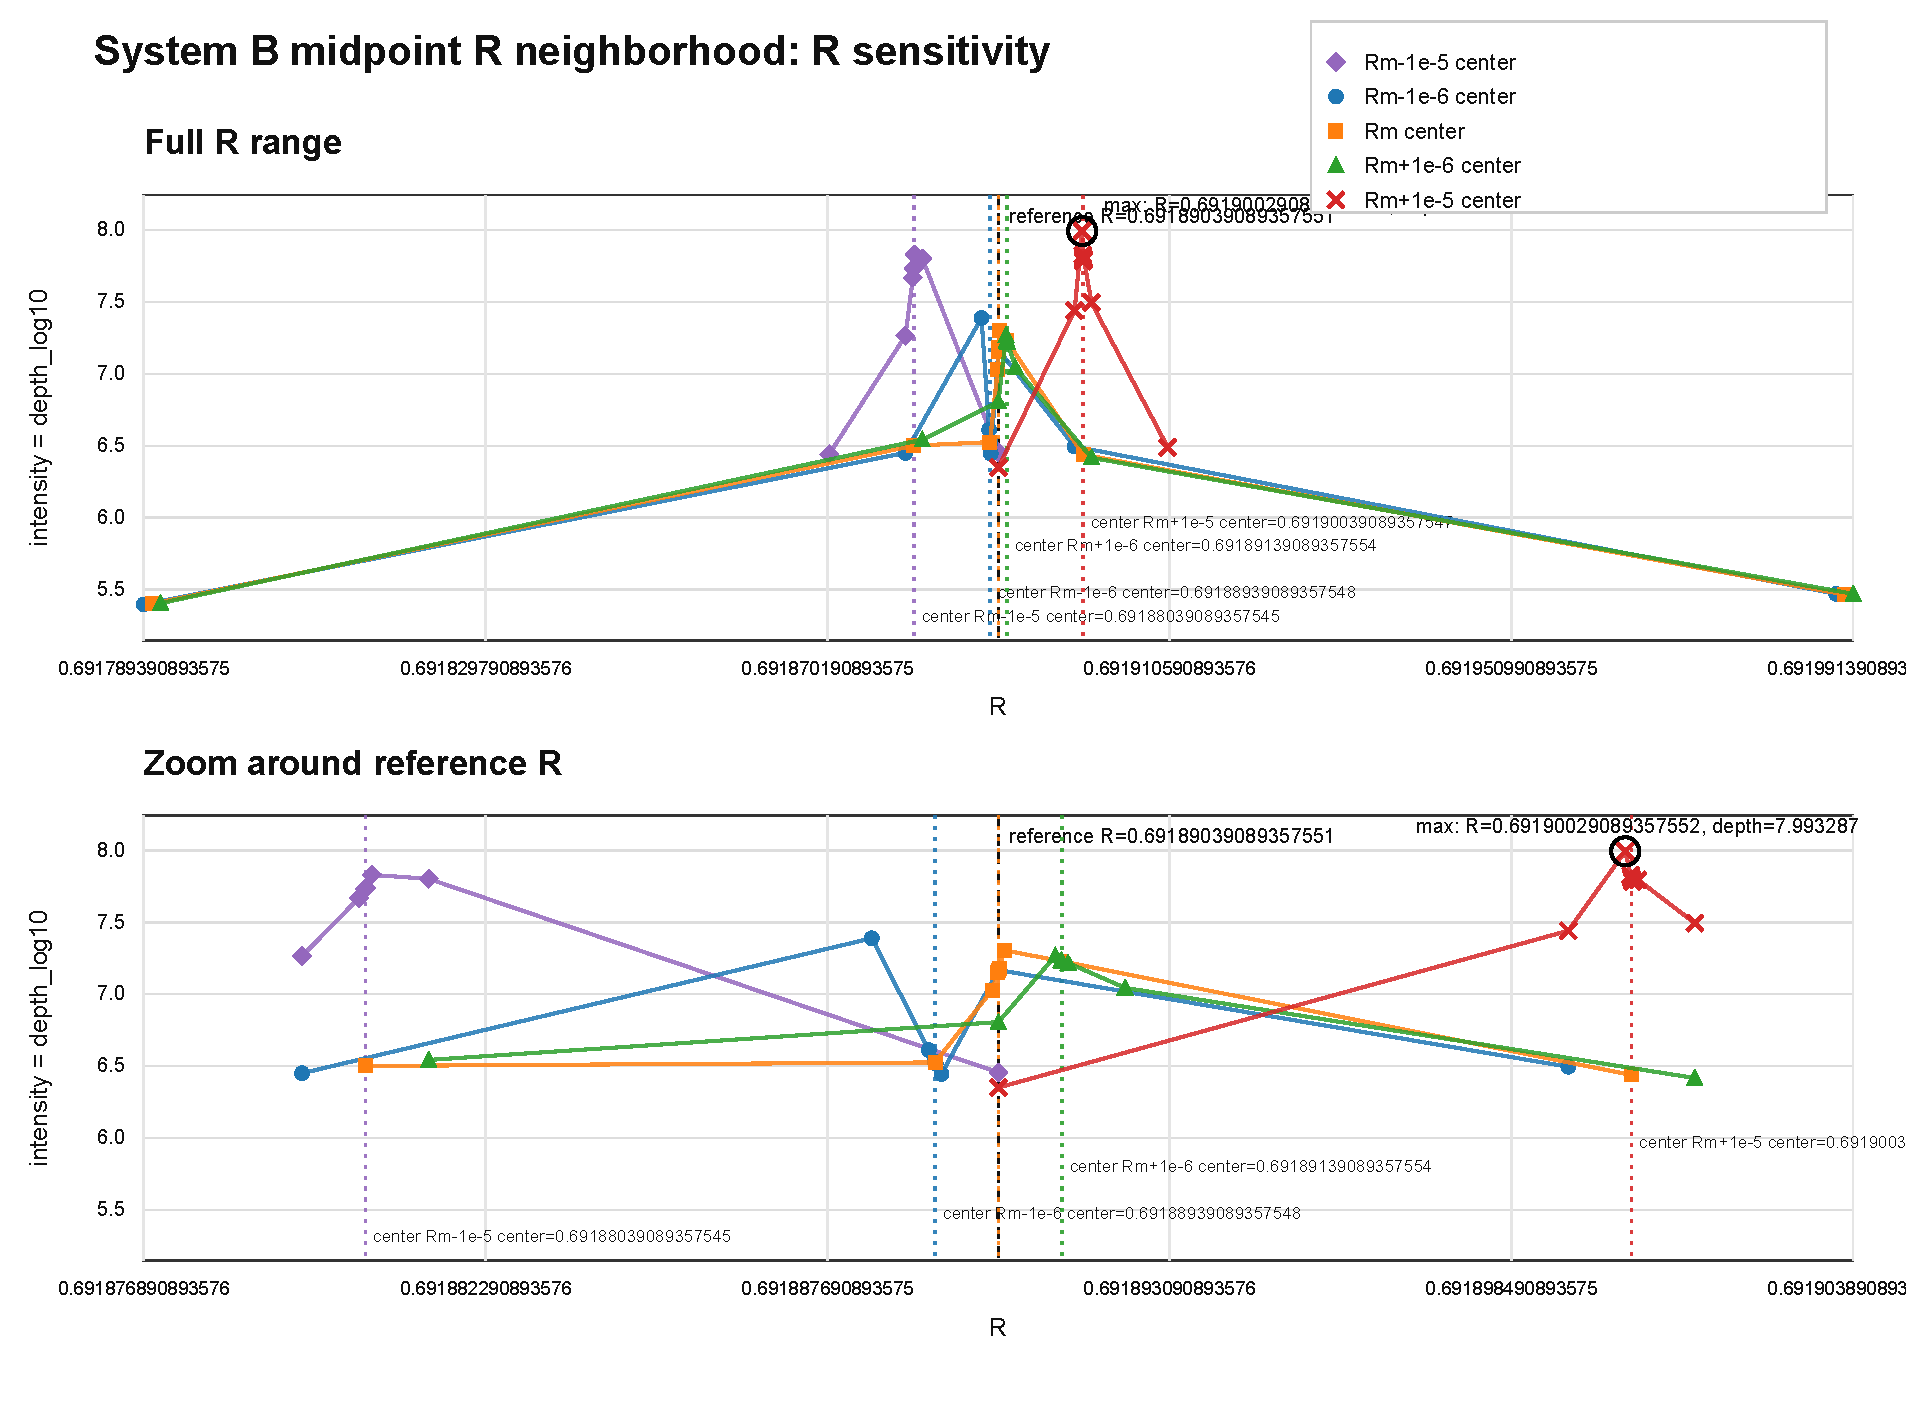
\includegraphics[keepaspectratio,alt={Intermediate R neighborhood}]{system_B_mid_R_sensitivity_depth_v1.pdf}}
\caption{Intermediate R neighborhood}
\end{figure}

\textbf{Figure 9.} Intermediate region between the low-energy and
high-energy sides. The candidate band is not strongly fixed at the
center and is difficult to read as a standard correspondence point.

The comparison is therefore read as follows:

\begin{Shaded}
\begin{Highlighting}[]
\NormalTok{Low{-}energy side:}
\NormalTok{  A strong candidate band exists at the R corresponding to alpha(0).}

\NormalTok{High{-}energy side:}
\NormalTok{  A deep candidate band exists near alpha(M\_Z\^{}2), but identity is not claimed.}

\NormalTok{Intermediate region:}
\NormalTok{  The correspondence candidate is weak.}
\end{Highlighting}
\end{Shaded}

\begin{center}\rule{0.5\linewidth}{0.5pt}\end{center}

\subsection{7. Discussion}\label{discussion}

\subsubsection{7.1 Why Are Harmonics
Necessary?}\label{why-are-harmonics-necessary}

In System A, the result was insensitive to the detailed amplitude,
phase, and wavelength of the additional harmonic.

However, when the additional harmonic was exactly zero, the
concentration near \texttt{R\_137}, or \texttt{G\_R≈sqrt(4πalpha(0))},
disappeared.

This suggests that the exchange-weight concentration may be related not
to the detailed shape of the harmonic waveform, but to the existence of
the additional degree of freedom itself.

In other words, in exchange scattering of closed phase systems, a
two-component system with only base waves and a system with at least one
additional harmonic degree of freedom may not be observing the same
reaction space.

\subsubsection{7.2 The Exchange-Weight Landscape Is Not
Single-Peaked}\label{the-exchange-weight-landscape-is-not-single-peaked}

The full-range sweep of System B did not produce a single candidate
band.

Candidate band 1 strongly corresponds to low-energy \texttt{alpha(0)}.

Candidate band 2 corresponds to \texttt{1/alpha≈129.394}, and lies near
the effective coupling at the Z-boson mass scale,
\texttt{1/alpha(M\_Z\^{}2)=128.946±0.015}.

The remaining candidate bands are shallower and are not strongly
connected to known standard-theory values at this stage.

This structure shows that \texttt{R≈0.7}, or \texttt{G\_R≈0.3}, is not
merely a single tuned value, but part of a multi-peak exchange-reaction
landscape in the metastable interface of the closed system.

\subsubsection{7.3 Candidate Correspondence with alpha, Not a Derivation
of
alpha}\label{candidate-correspondence-with-alpha-not-a-derivation-of-alpha}

The experiments in this paper do not derive the fine-structure constant
of the standard theory.

The essence of this paper is not the agreement with the fine-structure
constant itself, but the observation that a closed exchange map built
from a small set of axioms spontaneously selects a representative
state-exchange weight. The correspondence with the fine-structure
constant is treated as an observed result suggesting that the
intrinsically appearing exchange weight may be related to the
electromagnetic coupling in the real world.

Nevertheless, without inserting \texttt{alpha} from the outside, a
uniform scan of \texttt{R} produced its deepest candidate band at the
exchange weight corresponding to low-energy \texttt{alpha(0)}.

This suggests that the combination of exchange scattering, harmonic
degrees of freedom, and a metastable interface in a closed phase system
may not be unrelated to the electromagnetic coupling constant observed
in the standard theory.

The conclusion of this paper is therefore limited to:

\begin{Shaded}
\begin{Highlighting}[]
\NormalTok{In the exchange{-}weight landscape of exchange scattering in a closed phase system,}
\NormalTok{candidate bands that may correspond to the low{-}energy alpha}
\NormalTok{and the high{-}energy effective alpha of the standard theory appear.}
\end{Highlighting}
\end{Shaded}

\begin{center}\rule{0.5\linewidth}{0.5pt}\end{center}

\subsection{8. Claims Not Made in This
Paper}\label{claims-not-made-in-this-paper}

This paper does not claim:

\begin{Shaded}
\begin{Highlighting}[]
\NormalTok{that the fine{-}structure constant alpha has been derived;}
\NormalTok{that the standard theory has been replaced;}
\NormalTok{that candidate band 2 is exactly identical to alpha(M\_Z\^{}2);}
\NormalTok{that every fermion{-}scattering coefficient concentrates at the same exchange weight;}
\NormalTok{that the geometric origin of the harmonic degree of freedom has been fully explained.}
\end{Highlighting}
\end{Shaded}

What this paper shows is the numerical fact that alpha-correspondence
candidates appear in exchange-scattering experiments of closed phase
systems.

\begin{center}\rule{0.5\linewidth}{0.5pt}\end{center}

\subsection{9. Conclusion}\label{conclusion}

This paper used the exchange-scattering coefficient \texttt{R} as the
sweep coordinate and investigated, through two systems, the selection of
the representative state-exchange weight \texttt{G\_R=1-R}: a
localization-exchange model and a gray-cat metastable-interface model.

In System A, a single base harmonic did not produce a sharp
exchange-weight concentration. Once at least one additional harmonic
degree of freedom was present, the evaluation point of localization
exchange concentrated near \texttt{R=0.697177879...}, or equivalently
near \texttt{G\_R=1-R≈0.302822121}. This concentration was robust under
odd harmonics, even harmonics, mixed parity packets, reduced amplitude,
phase shifts, and wavelength shifts.

In System B, the minimal v5 implementation of the gray-cat metastable
interface swept

\begin{Shaded}
\begin{Highlighting}[]
\NormalTok{R = 0.686602902... to R = 0.702465367...}
\end{Highlighting}
\end{Shaded}

with

\begin{Shaded}
\begin{Highlighting}[]
\NormalTok{Delta R = 1.0e{-}7.}
\end{Highlighting}
\end{Shaded}

Seven candidate bands appeared. The deepest candidate band was

\begin{Shaded}
\begin{Highlighting}[]
\NormalTok{R = 0.697177902556148.}
\end{Highlighting}
\end{Shaded}

This agrees, within the seven-digit effective precision of the v5
experiment, with

\begin{Shaded}
\begin{Highlighting}[]
\NormalTok{R\_low = 0.697177879231003}
\end{Highlighting}
\end{Shaded}

obtained from the CODATA 2022 low-energy fine-structure constant by

\begin{Shaded}
\begin{Highlighting}[]
\NormalTok{R = 1 {-} sqrt(4 pi alpha).}
\end{Highlighting}
\end{Shaded}

The second candidate band was

\begin{Shaded}
\begin{Highlighting}[]
\NormalTok{R = 0.688363902556148,}
\end{Highlighting}
\end{Shaded}

corresponding to \texttt{1/alpha=129.394062925467}. This is not exactly
identical to the standard reference value of \texttt{alpha(M\_Z\^{}2)},
but is retained as a high-energy effective-coupling candidate.

Thus, in a closed phase-system exchange-scattering map, when a
metastable interface with harmonic degrees of freedom is read, candidate
bands of the representative state-exchange weight corresponding to the
fine-structure constant appear spontaneously.

\begin{center}\rule{0.5\linewidth}{0.5pt}\end{center}

\subsection{References}\label{references}

\subsubsection{Self-References}\label{self-references}

\begin{enumerate}
\def\labelenumi{\arabic{enumi}.}
\tightlist
\item
  Noriaki Kihara, \href{../20260710/基本公理系\%20v4.md}{Basic Axiom
  System v4}, 2026.
\item
  Noriaki Kihara,
  \href{../20260710/フェルミオン的逆相核による完全反射写像の干渉構成\%20v2.md}{Interference
  Construction of a Complete Reflection Map by a Fermion-Like
  Opposite-Phase Kernel v2}, 2026.
\item
  Noriaki Kihara,
  \href{../20260713/交換干渉散乱行列フェルミオン的衝突における低局在性・倍音移乗読出し実験仕様書\%20v1.md}{Experiment
  Specification for Low-Localization and Harmonic-Transfer Readout in
  Exchange-Interference Scattering-Matrix Fermion-Like Collisions v1},
  2026.
\item
  Noriaki Kihara,
  \href{../20260713/交換干渉散乱行列フェルミオン的衝突における低局在性・倍音移乗予備実験総括\%20v1.md}{Preliminary
  Summary of Low-Localization and Harmonic Transfer in
  Exchange-Interference Scattering-Matrix Fermion-Like Collisions v1},
  2026.
\item
  Noriaki Kihara,
  \href{../20260714/白猫黒猫灰色猫準安定界面におけるC弱読出しとD強観測選択予備実験総括\%20v1.md}{Preliminary
  Summary of C Weak Readout and D Strong-Observation Selection at the
  White-Cat, Black-Cat, and Gray-Cat Metastable Interface v1}, 2026.
\item
  Noriaki Kihara,
  \href{交換散乱係数R集中実験群_全体計画と評価方法_v1.md}{Overall Plan
  and Evaluation Method for the Exchange-Scattering Coefficient R
  Concentration Experiment Group v1}, 2026.
\item
  Noriaki Kihara,
  \href{系統A_局在性交換R近傍斉一スイープ実験仕様書_v1.md}{System A:
  Experiment Specification for Uniform R-Neighborhood Sweep in
  Localization Exchange v1}, 2026.
\item
  Noriaki Kihara,
  \href{系統B_灰色猫準安定界面R近傍スイープ実験仕様書_v1.md}{System B:
  Experiment Specification for R-Neighborhood Sweep of the Gray-Cat
  Metastable Interface v1}, 2026.
\item
  Noriaki Kihara, \href{標準理論でのα.md}{alpha in the Standard Theory},
  2026.
\end{enumerate}

\subsubsection{External References}\label{external-references}

\begin{enumerate}
\def\labelenumi{\arabic{enumi}.}
\setcounter{enumi}{9}
\tightlist
\item
  Peter J. Mohr, David B. Newell, Barry N. Taylor, Eite Tiesinga,
  ``CODATA Recommended Values of the Fundamental Physical Constants:
  2022'', arXiv:2409.03787, 2024. https://arxiv.org/abs/2409.03787
\item
  National Institute of Standards and Technology, ``Fundamental Physical
  Constants'', https://physics.nist.gov/constants
\item
  Alexander Keshavarzi, Daisuke Nomura, Thomas Teubner, ``The muon g-2
  and alpha(M\_Z\^{}2): a new data-based analysis'', arXiv:1802.02995,
  2018. https://arxiv.org/abs/1802.02995
\end{enumerate}

\begin{center}\rule{0.5\linewidth}{0.5pt}\end{center}

\subsection{Appendix A. Main Outputs Used for
Reproduction}\label{appendix-a.-main-outputs-used-for-reproduction}

{\def\LTcaptype{none} % do not increment counter
\begin{longtable}[]{@{}
  >{\raggedright\arraybackslash}p{(\linewidth - 2\tabcolsep) * \real{0.5000}}
  >{\raggedright\arraybackslash}p{(\linewidth - 2\tabcolsep) * \real{0.5000}}@{}}
\toprule\noalign{}
\begin{minipage}[b]{\linewidth}\raggedright
Type
\end{minipage} & \begin{minipage}[b]{\linewidth}\raggedright
File
\end{minipage} \\
\midrule\noalign{}
\endhead
\bottomrule\noalign{}
\endlastfoot
System A N-series &
\texttt{system\_A\_localization\_exchange\_R\_sweep\_result\_v1/odd\_kernel\_N\_1\_2\_3\_5\_15\_63\_report\_v1.md} \\
System A even packet &
\texttt{system\_A\_localization\_exchange\_R\_sweep\_result\_v1/even\_packet\_A1\_B1\_2\_4\_6\_report\_v1.md} \\
System A mixed packet 1 &
\texttt{system\_A\_localization\_exchange\_R\_sweep\_result\_v1/alternating\_packet\_1\_A1\_B1\_2\_3\_4\_5\_report\_v1.md} \\
System A mixed packet 2 &
\texttt{system\_A\_localization\_exchange\_R\_sweep\_result\_v1/alternating\_packet\_2\_A1\_B1\_3\_4\_5\_6\_report\_v1.md} \\
System A zero-amplitude control &
\texttt{system\_A\_localization\_exchange\_R\_sweep\_result\_v1/amp000\_B12/system\_A\_amp000\_B12\_custom\_packet\_A1\_B1-2-w-1-0\_Rdefault\_C256\_report\_v1.md} \\
System B full-range candidate bands &
\texttt{System\ B\ 全域Rスイープ候補帯一覧.md} \\
System B low-energy neighborhood &
\texttt{System\ B\ 低エネルギー標準α近傍R感度一覧.md} \\
System B high-energy neighborhood &
\texttt{System\ B\ 高エネルギー標準α近傍R感度一覧.md} \\
System B intermediate region &
\texttt{System\ B\ 中間R近傍R感度一覧.md} \\
\end{longtable}
}

\end{document}
